\documentclass[a4paper]{jpconf}

% graphics packages
\usepackage{graphicx}
\usepackage{stackengine}
\usepackage{subfigure}
\usepackage{float}
\usepackage{placeins}

% algorithm packages
%\usepackage{algpseudocode}
%\usepackage{algorithm}
\usepackage{amsmath}

% symbols
\usepackage{gensymb}

% reference packages
\usepackage[hidelinks]{hyperref}
\usepackage{cleveref}
\usepackage{url}

% formatting packages
\usepackage{enumitem}
\usepackage{flafter}
\usepackage{booktabs}

\graphicspath{{./final_images/}}

% editing packages
\usepackage{todonotes}

\begin{document}

\title{Wake Expansion Continuation: \large{Multi-modality reduction in the wind farm layout optimization problem}}

\author{J~J~Thomas, S~McOmber, and A~Ning}
\address{Department of Mechanical Engineering,
Brigham Young University, Provo, Utah, USA}
\ead{jaredthomas@byu.net}

\begin{abstract}
	This paper presents a process using an approach related to  continuation optimization methods for reducing multi-modality in the wind farm layout optimization problem, referred to as Wake Expansion Continuation (WEC). The reduction in multi-modality is achieved by starting with an increased wake spread, while maintaining normal velocity deficits at the center of the wakes, and then reducing the wake spread for each of a series of optimization runs until the standard wake spread is used. Two optimization cases were tested, one with 16 turbines and one with 38 turbines, by optimizing from 200 different starting positions with a gradient-based method, a gradient-free method, and a gradient-based method using WEC. Results using WEC show a $4\%$ mean optimized annual energy production (AEP) improvement compared to gradient-based optimization without WEC for both test cases. A gradient-free algorithm had a mean optimized AEP that was $1\%$ higher than WEC for the 16-turbine case, but WEC resulted in a $10\%$ higher mean optimized AEP compared to a gradient-free optimization method for the 38-turbine problem. These results are specific to the test cases and may not be generally representative.
\end{abstract}

\section{Introduction}

The difficulty of solving the wind farm layout optimization (WFLO) problem is primarily due to the large number of variables and constraints required for realistic problems and the multi-modal nature of the problem's design space. Gradient-free optimization methods are the most common methods used to solve the WFLO problem. However, gradient-free methods have been shown to have reduced performance with high dimensional problems \cite{rios2013-grad-free-comparison}. The WFLO problem scales quickly to high dimensions as the number of turbines is increased. Gradient-based optimization methods are well suited for high dimensional problems. Gradient-based methods are not widely used for WFLO problems, but are gaining interest due to their relatively low computational cost and their ability to handle many variables and constraints. However, gradient-based methods are highly susceptible to local optima \cite{acero2014}. Despite this weakness, they have been shown to find good solutions to WFLO problems \cite{fleming2015, guirguis2016, gebraad2017-Maximization-Annual}.  

Many techniques have been presented to make the WFLO problem more tractable, including discretization, multi-start, re-parameterization, and hybrid approaches. Discretization techniques, used with gradient-free methods, attempt to simplify the problem by reducing the number of possible solutions \cite{mosetti1994, grady2005}. Through discretization, the number of possible turbine locations within a wind farm can be reduced from infinite to something on the order of hundreds of locations. However, discretization disregards any locations that are not pre-selected, and can thus preclude this approach from finding even a local optimum. It is also possible that constraints on variables other than position may render the discretized optimization problem intractable. Multi-start approaches involve running many optimizations of one problem with different starting points \cite{gonzalez2014}. This approach reduces the sensitivity of gradient-based optimization methods to local optima. Re-parameterization approaches seek to reduce the complexity of the problem by defining the wind farm with just a few variables, such as row spacing, column spacing, grid rotation, etc.~as done in \cite{stanley2020}. Hybrid approaches combine gradient-based and gradient-free algorithms iteratively \cite{rethore2014,graf2016, mittal2017}, and, depending on the problem size, can yield result quality comparable to multi-start approaches \cite{rethore2014}. While each of these techniques yield improved results, there is still need for improvement because current methods have a wide spread in the quality of results, are highly dependent on starting locations, artificially limit the design space, and/or cannot be applied in realistic wind farm optimization scenarios. These limitations indicate that there is need for better optimization methods that avoid local optima, whether real or imposed by the approach itself.

Current methods seek to avoid local optima by searching the existing design space more broadly. This approach becomes intractable for large optimization problems with many variables and constraints. To address this issue, we propose a process for use with gradient-based optimization algorithms that temporarily reduces the number and magnitude of local optima using a continuation optimization approach such as the method discussed in \cite{mobahi2015}. However, while continuation optimization uses a numerical approximation of the design space, our proposed process takes advantages of the physical properties of the design space directly. We will refer to the new process as Wake Expansion Continuation, or WEC.

In the following sections we (1) describe the WEC method generally, (2) discuss the models we used to test WEC, (3) demonstrate how to apply WEC to two different wake models, and (4) asses the performance of WEC compared with other methods in three case studies.

\section{Wake Expansion Continuation}\label{sec:dsrop}
The two primary characteristics that simple wake models seek to capture are wake diameter and velocity deficit. These characteristics in turn largely determine the shape of the wind farm layout design space. The fluctuations of wind speed as turbines move in and out of the wakes during optimization are primarily responsible for the multi-modal nature of the WFLO problem. 

During optimization, the spaces between wakes translate to locally optimal locations for turbines. However, it is often the case that there are more optimal turbine locations that are not found by the optimizer because the turbines are effectively stuck in locally optimal locations. The proposed WEC method seeks to overcome the problem of local optima by temporarily reducing the multi-modality of the design space. 

The WEC method is somewhat analogous to Gaussian continuation optimization. In Gaussian continuation optimization, the design space is approximated using a series of Gaussian radial basis functions. When optimization is performed, the standard deviations of the radial basis functions starts at a relatively high value and slowly decreases until the original standard deviation is reached \cite{mobahi2015}. Increasing the standard deviation of the basis functions has the effect of causing the various basis functions to blend in to each other, effectively removing the local optima and providing a relatively convex design space to the optimization algorithm. Slowly returning the standard deviation to the original value allows the optimization algorithm to adjust for any shift in the global optimum due to the blending of the basis functions and avoid any nearby local optima. 

WEC works in a manner similar to Gaussian continuation optimization, except that because wind turbine wakes are roughly Gaussian-shaped, the Gaussian basis functions are built in to the model directly rather than used to approximate the model. Other key differences are that the basis function in WEC are not radial, and the changing locations of the Gaussian functions during the WFLO mean that we cannot guarantee convergence to the global optimum. However, the use of the WEC method does significantly improve the optimization results, as will be shown.

\subsection{How WEC works}

The WEC method can be explained in three basic steps:
\begin{enumerate}[label=\arabic*)]
	\item Determine how the wake diameter and wake deficit are controlled for the selected wake model.
    \item If necessary, add a factor to the model such that the wake diameter can be directly controlled without significantly altering the wake deficit in the center of the wake. Avoiding altering the wake deficit in the center of the wake mimics the behavior of increasing the standard deviation for a Gaussian distribution as done in \cite{mobahi2015}.
    \item Run a series of optimizations such that the wake diameter is larger than normal for the first optimization, and then reduces with each subsequent optimization until the wake spread is no longer altered from the original model. Each optimization after the first should be hot-started using the result of the previous optimization.
\end{enumerate}

By spreading the wakes, we can effectively fill in the gaps between wakes so that a gradient-based optimization algorithm can bypass local optima and proceed to a better solution. Another way of thinking about this is that by spreading the wakes, more turbines see the influence of each wake, which provides more information to the gradient-based optimization algorithm about the design space through the Jacobian. 

\subsection{Three ways to expand the wake}\label{sec:wecmethods} 
To apply the wake expansion technique to the wind farm layout optimization problem, we need to determine the best way to expand the basis functions, or wake diameter in this case. We have investigated three ways of spreading the wake: (1) increasing the wake spreading angle (WEC-A), (2) multiplying the initial wake diameter (WEC-D), and (3) a hybrid of 2 and 3 that is accomplished by multiplying the wake diameter at an estimated point of far wake onset and allowing the wake to follow an angled line from the initial wake diameter to the expanded far wake diameter (WEC-H). The impact on the wake shape of each of these three methods of expanding the wake are shown in \cref{fig:wec-methods}.

\begin{figure}[h]
	\centering
	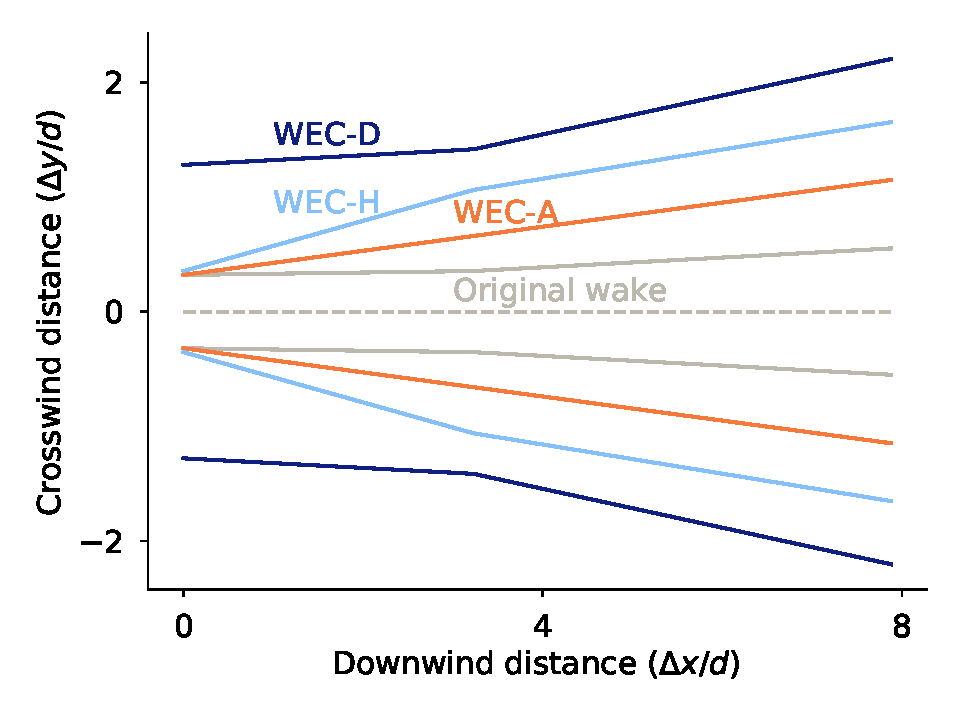
\includegraphics[width=0.6\textwidth,trim={0, 0, 0, 2.0}]{wec-methods}
	\caption{The impact on wake shape of expanding the wake by increasing the spreading angle (WEC-A), the diameter (WEC-D), or a downstream diameter that also changes the near wake spreading angle (WEC-H). The relative amount of expansion in the figure is for convenience in comparing the WEC methods. The actual amount of expansion is variable for all methods.}
	\label{fig:wec-methods}
\end{figure}

\section{Wake and Wind Farm Models}
Because of the general nature of the proposed method, it could theoretically be applied to a range of wake models. In this study we have applied WEC to the 2016 version of the Bastankhah and Port\'e-Agel wake model \cite{bastankhah2016} and the cosine version of the Jensen model \cite{jensen1983}. We also used various other models necessary for combining wakes and calculating wind farm AEP.

\subsection{The Bastankhah and Port\'e-Agel Wake Model}
In the Bastankhah and Port\'e-Agel wake model, the two primary characteristics of the wakes, wake deficit and wake diameter, are particularly easy to isolate. This, along with the smoothness and differentiability of the model, make it a good example for demonstrating WEC. We used the Bastankhah and Port\'e-Agel wake model, as defined in \cref{eq:bpa} \cite{bastankhah2016}, along with the Niayifar and Port\'e-Agel wind farm model \cite{niayifar2016}.
%
\begin{equation}
	\frac{\Delta \bar{u}}{\bar{u}_{\infty}} = \Bigg(1-\sqrt{1-\frac{C_T \cos{\gamma}}{8 \sigma_y \sigma_z/d^2}}~\Bigg) \exp{\bigg(-0.5\Big(\frac{y-\delta}{\sigma_y}\Big)^2\bigg)}\exp{\bigg(-0.5\Big(\frac{z-z_h}{\sigma_z}\Big)^2\bigg)}
	 \label{eq:bpa}
\end{equation}
%
Where $\Delta \bar{u} / \bar{u}_{\infty}$ is the normalized wake velocity deficit, $C_T$ is the thrust coefficient, $\gamma$ is the upstream turbine's yaw angle with respect to the inflow direction, $y-\delta$ and $z-z_h$ are the distances of the point of interest from the wake center in the cross-stream horizontal and vertical directions respectively, and $\sigma_y$ and $\sigma_z$ are the standard deviations of the wake deficit in the cross-stream horizontal and vertical directions as defined in \cref{eq:sigmay,eq:sigmaz}.
%
\begin{equation}\label{eq:sigmay}
	\sigma_y = k_y (\Delta x - x_0) + \frac{d \cos{\gamma}}{\sqrt{8}}
\end{equation}
%
\begin{equation}\label{eq:sigmaz}
	\sigma_z = k_z (\Delta x - x_0) + \frac{d}{\sqrt{8}}
\end{equation}
%
In \cref{eq:sigmay,eq:sigmaz}, $\Delta x$ is the downstream distance from the turbine generating the wake to the point of interest, $x_0$ is the length of the wake potential core, $d$ is the diameter of the turbine generating the wake, and $k_y$ and $k_z$ are determined as a function of turbulence intensity ($I$) as defined in \cref{eq:kstar}\cite{niayifar2016}.
%
\begin{equation}\label{eq:kstar}
	k^* = 0.3837I + 0.003678
\end{equation}
%
While the Niayifar and Port\'e-Agel wind farm model calculates $k^*$ based on local turbulence intensity at each turbine, the local turbulence intensity calculations introduce more local optima and discontinuities. For this reason, we chose to ignore local turbulence intensity while using WEC. However, a smooth version of the local turbulence intensity was used in a final optimization step following all WEC steps in studies performed using WEC with the Bastankhah and Port\'e-Agel wake model and gradient-based optimization methods. While local turbulence intensity does impact the accuracy of the power predictions, it does not alter the general trends within the design space, and most simple wake models ignore local turbulence intensity. 

The Gaussian shape of the Bastankhah and Port\'e-Agel wake model is well suited for gradient-based optimization because it is smooth, continuous, and has no flat regions. However, in the near wake, the model can either be flat, which can cause premature convergence, or be undefined, which can cause optimizations to fail. Because no turbines will be placed in this region of the wake in the final optimized layout, the accuracy of the model in the near wake is second in importance to wake shape and continuity. 

We define our near wake model using the location where the original model first begins to be defined, $x_d$, derived in \cite{thomas2019-les-validation} and reproduced in \cref{eq:xd}.
%
\begin{equation}\label{eq:xd}
x_d = x_0 + \frac{d\Bigg[k_y+k_z\cos{\gamma} - \sqrt{[k_y+k_z\cos{\gamma}]^2-4k_y k_z[C_T-1]\cos{\gamma}}\Bigg]}{2k_y k_z\sqrt{8}}
\end{equation}
%
We find the standard deviation of the wake at the point $x_d$ as shown in \cref{eq:sigmayd}
%
\begin{equation}\label{eq:sigmayd}
\sigma_{yd} = k_y (x_d - x_0) + \frac{D_r \cos{\gamma}}{\sqrt{8}}
\end{equation}
%
We then use the definition of the wake spread at the point of discontinuity to provide an estimate for the wake spread and velocity deficit at the rotor hub. This is an important assumption because we need to have some slope in the wake spread between the rotor hub and the point of far wake onset for more effective gradient-based optimization. With the assumption that $\sigma_{yd}$ is the value of the wake spread at the rotor hub, we can define the slope of the near wake, $k_{y_{NEAR}}$, as shown in \cref{eq:kynear}.
%
\begin{equation}\label{eq:kynear}
k_{y_{NEAR}} = \frac{\sigma_{yo}-\sigma_{yd}}{x_o}
\end{equation}
For more details on near wake approximation of the Bastankhah and Port\'e-Agel wake model used in this study, please see \cite{thomas2019-les-validation}.

\subsection{The Jensen Cosine Wake Model}
The Jensen cosine wake model is a variant of the popular "top hat" model often referred to as the Jensen model. The cosine version simply multiplies the top hat shape with a factor that changes the cross wake deficit shape to follow a cosine curve. The Jensen cosine wake model is shown in \cref{eq:JensenVelocityDeficit}.

% Equation for the Jensen Cosine velocity deficit.
\begin{equation}
\frac{ \bar{u}}{\bar{u}_\infty} = 1 - 2a \bigg(\frac{r_0}{r_0 + \alpha \Delta x} \bigg)^2 f_\theta 
\label{eq:JensenVelocityDeficit}
\end{equation}
%
In \cref{eq:JensenVelocityDeficit}, $\bar{u}$ represents the wind velocity at a distance $\Delta x$ downstream of the waking turbine, $\bar{u}_\infty$ represents the free-stream wind velocity, $r_0$ represents the radius of the wind turbine, $\alpha$ represents the wake entrainment constant \cite{jensen1983}, $a$ represents the axial induction (for which we assumed an ideal value of $a = 1/3$), and $f_\theta$ is the cosine factor defined in \cref{eq:JensenCosineAdjustment}.
%
% Enter the Cosine Adjustment Equation to Jensen's Wake Model.
\begin{equation}
f_\theta = \frac{1 + cos(n\theta)}{2}
\label{eq:JensenCosineAdjustment}
\end{equation}
%
In \cref{eq:JensenCosineAdjustment},  $\theta$ is the angle from the wake center line to the point of interest measure at the wake vertex a distance $z$ upstream of the wind turbine, $n$ represents an adjustment factor derived from the wake spreading angle $\beta$, as shown in \cref{fig:JensenDiagrams}. The value for $n$ can be calculated as in \cref{eq:nFactor}, where $\beta$ is in radians.
%
% Equation to determine the factor n in the Jensen Cosine factor.
\begin{equation}
n = \pi / \beta
\label{eq:nFactor}
\end{equation}
%
The wake spreading angle used in this work, and by Jensen, was $\beta = 20 \degree$  \cite{jensen1983}. See \cref{fig:JensenDiagrams} for a diagram showing the overhead geometry of the Jensen Cosine model.
%
% New diagram that combines two subfigures into a single figure.
\begin{figure}[h!]
	\centering
	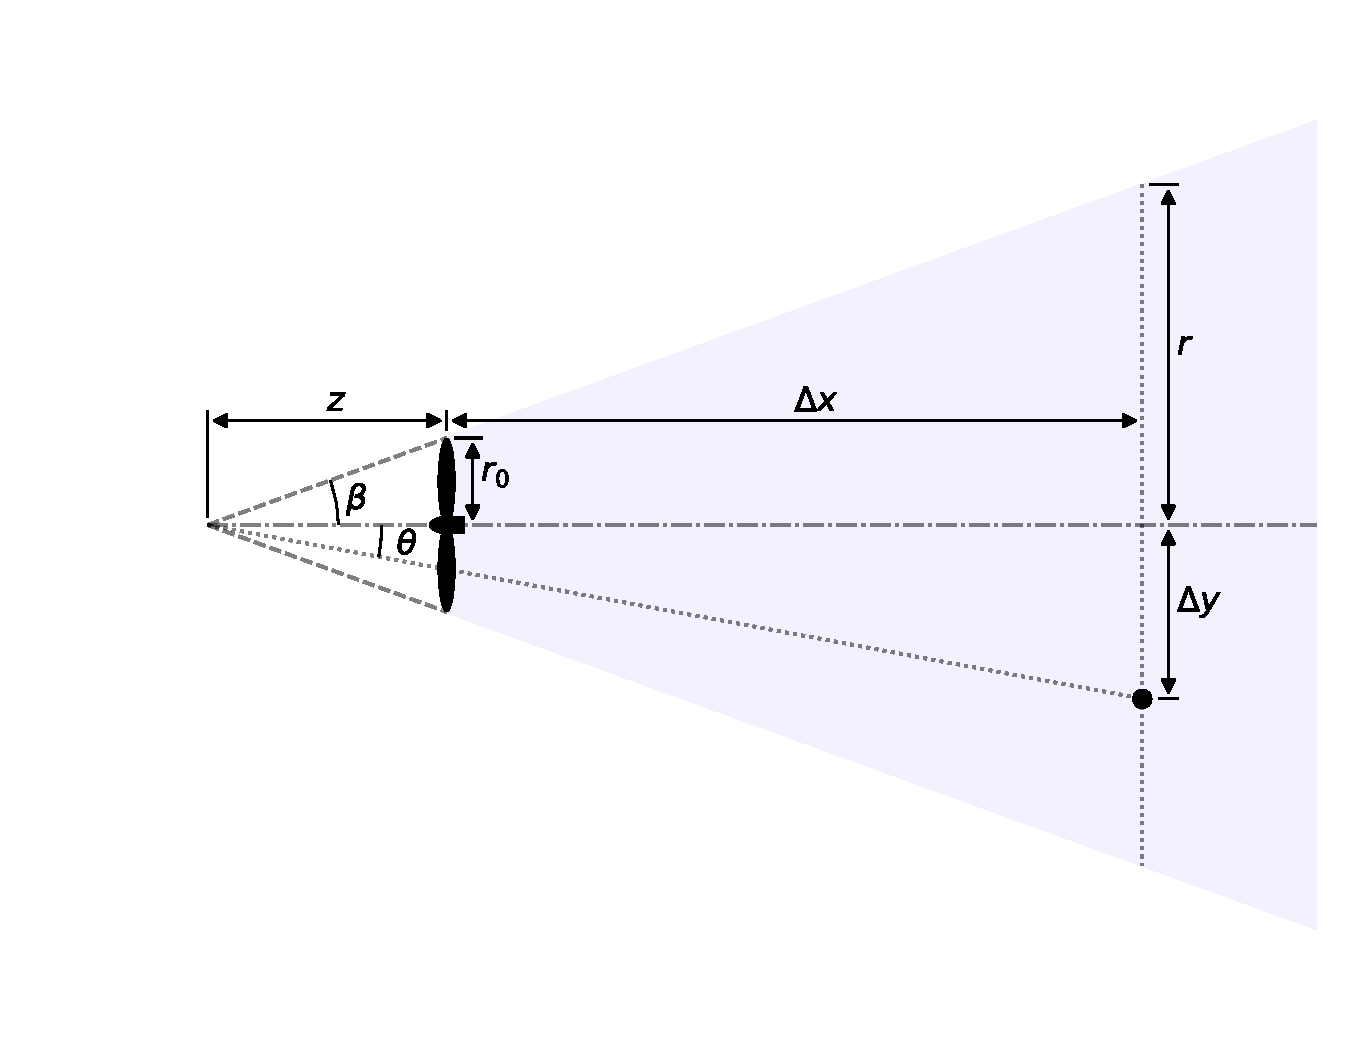
\includegraphics[width=0.6\textwidth,trim={3.5cm 2cm 0cm 2cm} ]{jensen_diagram}
	\caption{Diagram showing the overhead geometry of the Jensen cosine wake model. The wind is blowing to the right. The dashed line down the middle represents the center line of the wake. The large black dot represents any given point of interest.}
	\label{fig:JensenDiagrams}
\end{figure}

\subsection{Turbine Model}
We based our turbines on the Vestas V-80 2MW wind turbine for all studies in this paper. The values of $C_P$ and $C_T$ were based on a linear interpolation of the power and thrust coefficient curves presented in \cite{niayifar2016} and shown in \cref{fig:cp,fig:ct}. The other turbine specifications are provide in \cref{tab:v80}. The $C_T$ curve was only used with the Bastankhah and Port\'e-Agel wake model. We used a constant axial induction value of 1/3 for the Jensen cosine wake model.
%
\begin{figure}[htp]
	\centering
	\begin{minipage}[t]{0.48\textwidth}
		\centering
		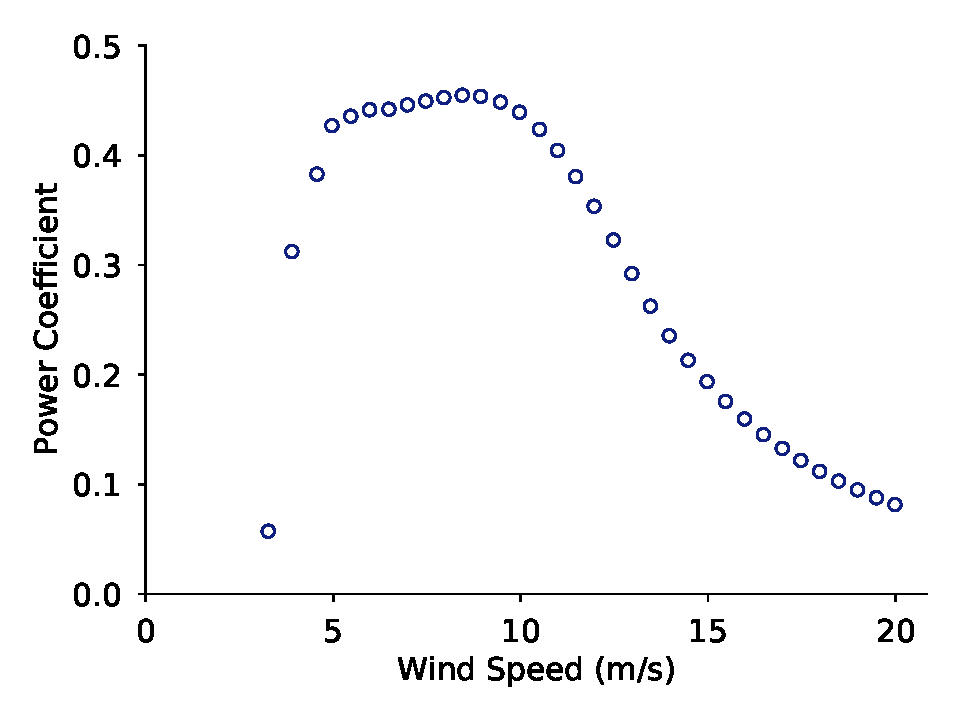
\includegraphics[width=\textwidth, trim={0cm 0cm 0cm 0cm}, clip]{cp_curve_v80}
		\caption{$C_P$ curve for the Vestas V80 2MW wind turbine \cite{niayifar2016} }
		\label{fig:cp}
	\end{minipage}\hspace{1pc}%
	\begin{minipage}[t]{0.48\textwidth}
		\centering
		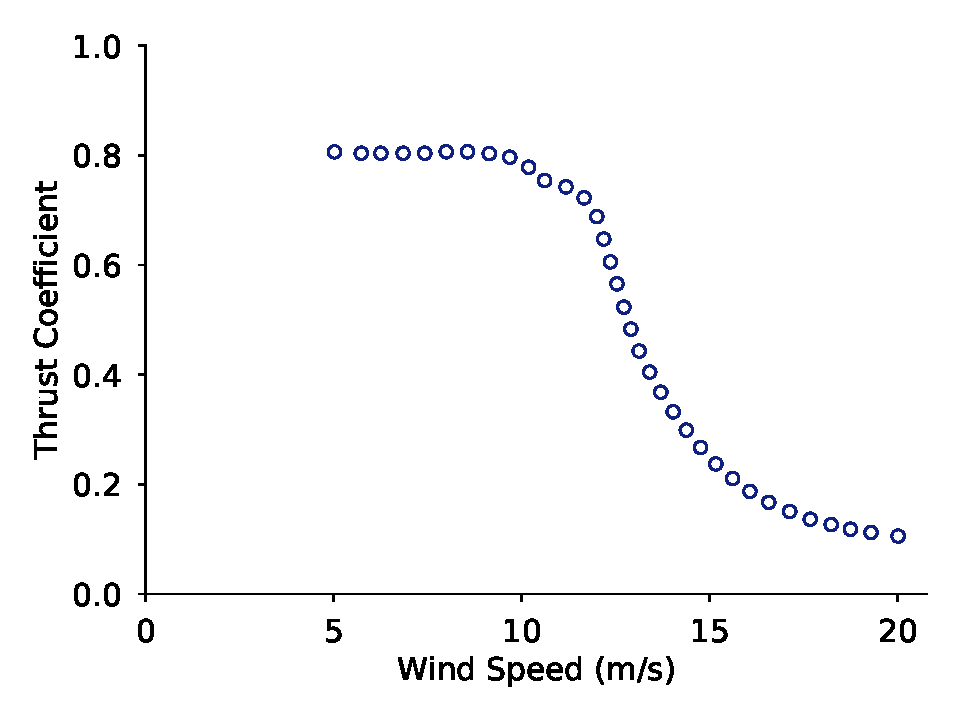
\includegraphics[width=\textwidth]{ct_curve_v80.pdf}
		\caption{$C_T$ curve for the Vestas V80 2MW wind turbine \cite{niayifar2016}}
		\label{fig:ct}
	\end{minipage} 
\end{figure}
%
\begin{table}
	\caption{Turbine Specifications}
	\label{tab:v80}
	\centering
	\begin{tabular}{l l}
		\br
		Rotor Diameter & 80.0 m\\
		Hub Height & 70.0 m \\
		Cut-in Speed & 4.0 m/s\\
		Cut-out Speed & 25.0 m/s \\
		Rated Speed & 16.0 m/s \\
		Rated Power & 2.0 MW \\
		Generator Efficiency & 0.944 \\
		\br
	\end{tabular}
\end{table}

\subsection{Other Models}
We combined the wake deficits using a linear combination method as discussed in \cite{niayifar2016} with the Bastankhah and Port\'e-Agel wake model, and a sum of squares method with the Jensen wake model as discussed in \cite{katic1986}. We used a reference height of 80 m for all wind speed measurements and adjusted to different heights with a power law and a wind shear exponent of 0.31 as shown in \cref{eq:shear}. 
%
\begin{equation} \label{eq:shear}
u = u_r\bigg[\frac{z}{z_r}\bigg]^\psi
\end{equation}
%
In \Cref{eq:shear}, $u_r$ is the reference wind speed, $z$ is the height of interest, $z_r$ is the height at which $u_r$ was measured, and $\psi$ is the shear exponent.

To save computation time, the inflow wind speed at each turbine was approximated using a single sample at the wind turbine hub location. Individual turbine inflow wind velocities, $U_i$, were solved consecutively from upstream to downstream for each wind state (direction and speed combination) for the Bastankhah and Port\'e-Agel wake model, but in no particular order for the Jensen cosine model. The power output of each turbine was then calculated based on \cref{eq:power}
%
\begin{equation}\label{eq:power}
P_i = \frac{1}{2}\rho A_{r,i}C_P U_i^3
\end{equation}
%
where $\rho$ is the air density, $A_{r,i}$ is the rotor-swept area of turbine $i$, and $C_P$ is the power coefficient. We calculated annual energy production (AEP) as shown in \cref{eq:aep}.

\begin{equation} \label{eq:aep}
AEP = (24)(365)\sum_{j=1}^{n_d} \bigg( p_j \sum_{i=1}^{n_t} P_i \bigg)  
\end{equation}

 In \cref{eq:aep}, $n_d$ is the number of wind directions, or states, $p_j$ is the probability of wind for a given state (direction and speed), and $n_t$ is the number of wind turbines.

\section{Implementation Details and Optimization Algorithms}
The code for each wake model was written in Fortran and wrapped in python. In this work, optimization problems were set up and solved in OpenMDAO \cite{gray2010_OpenMDAO} using two optimization algorithms, SNOPT and ALPSO. SNOPT is a gradient-based sparse non-linear optimization algorithm \cite{gill2005}. ALPSO is a particle swarm algorithm that uses an augmented Legrangian approach to handle constraints \cite{jansen2011_alpso}. Both algorithms were used through pyOptSparse \cite{perez2012a}. We obtained exact gradients for the Bastankhah and Port\'e-Agel wake model using algorithmic differentiation provided by Tapenade \cite{tapenade2013}. Gradients for the Jensen cosine wake model were obtained through a central difference approach. 

SNOPT was run with a convergence tolerance of 1E-4. The objective and constraints were scaled to be on the order of 1. ALPSO was run using the default parameters provided in pyOptSparse \cite{wu2020} with a few exceptions. First, the craziness velocity was set to be $1E-2$ as this value resulted in increased performance compared to the default value across all the cases we tested. We tried adjusting the initial particle velocity, but found no difference in results for the cases tested. As demonstrated in \cite{jansen2011_alpso}, we tested a series of values for inner iteration number and found that the inner iteration count had a large impact on the end results and convergence rates for all cases tested. We used different inner iteration counts for each case study, but held the number of function calls relatively constant at about 20000 as all cases appeared converged after this many function calls regardless of the number of inner iterations. We used a constant population seed of 1.0 while testing inner iteration counts. The number of outer iterations was determined based on the number inner iterations and desired function call cap for each case. The ALPSO convergence history for each case study with varied inner iteration counts is shown in \cref{fig:alpso-ii-16-20,fig:alpso-ii-38-12}. The objective and design variables were all scaled to be between -1 and 1.  All optimization runs using ALPSO had a population size of 30.

\begin{figure}[htp]
	\centering
	\begin{minipage}[t]{0.48\textwidth}
		\centering
		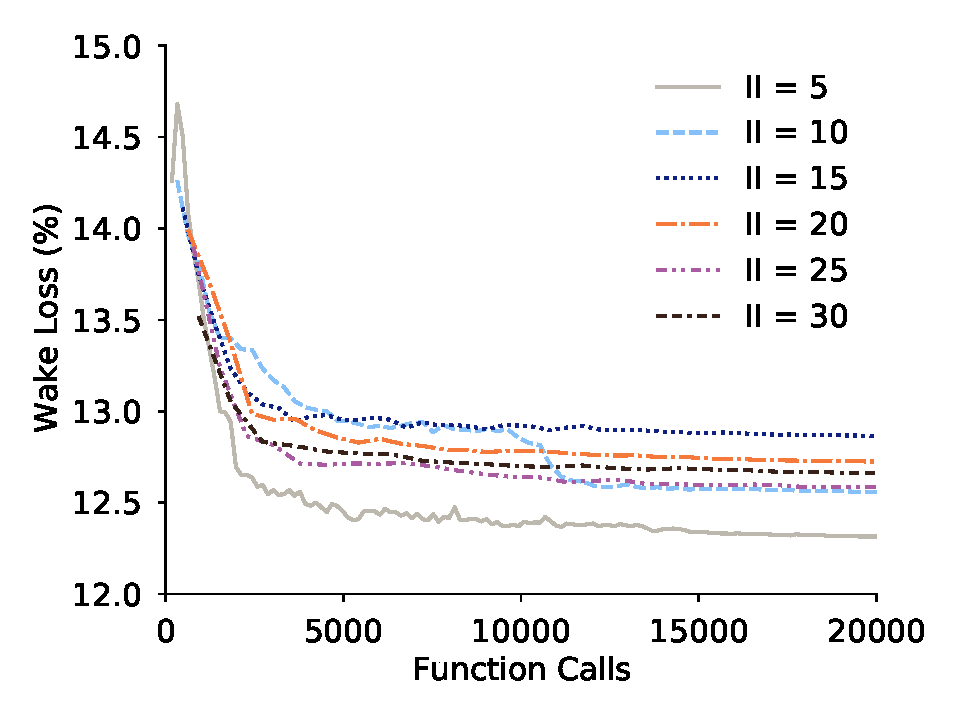
\includegraphics[width=\textwidth, trim={0cm 0cm 0cm 0cm}, clip]{tests/alpso_test_16turbs_20dirs.pdf}
		\caption{Comparing ALPSO convergence history for 16 turbines, 20 directions, and varying numbers of inner iterations.}
		\label{fig:alpso-ii-16-20}
	\end{minipage}\hspace{1pc}%
	\begin{minipage}[t]{0.48\textwidth}
		\centering
		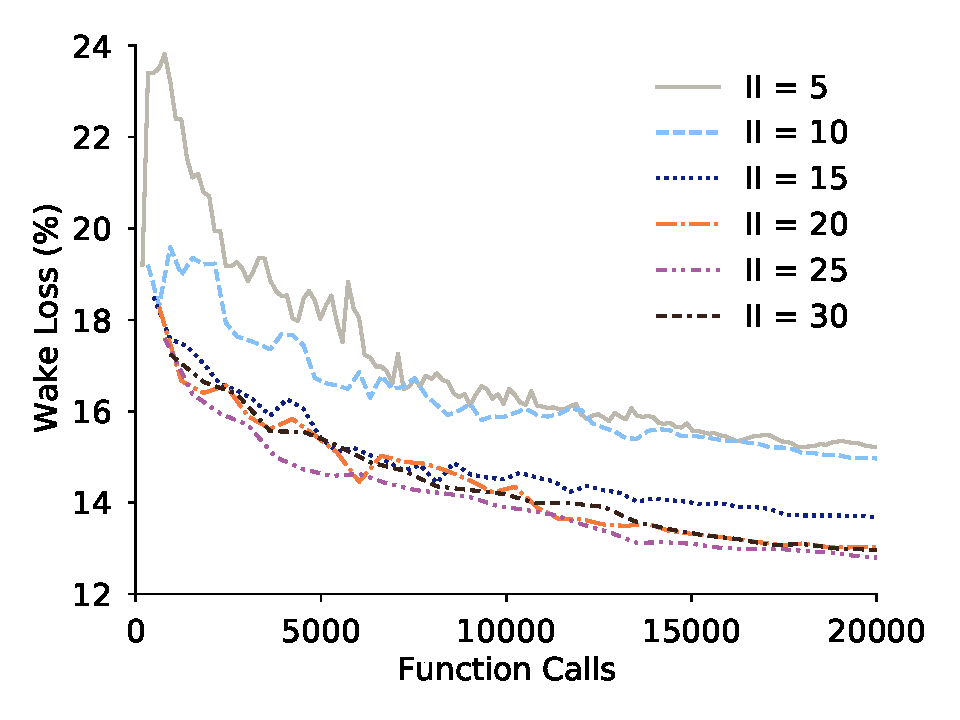
\includegraphics[width=\textwidth]{tests/alpso_test_38turbs_12dirs.pdf}
		\caption{Comparing ALPSO convergence history for 38 turbines, 12 directions, and varying numbers of inner iterations.}
		\label{fig:alpso-ii-38-12}
	\end{minipage} 
\end{figure}
\begin{figure}[htp]
	\centering
	\begin{minipage}[t]{0.48\textwidth}
		\centering
		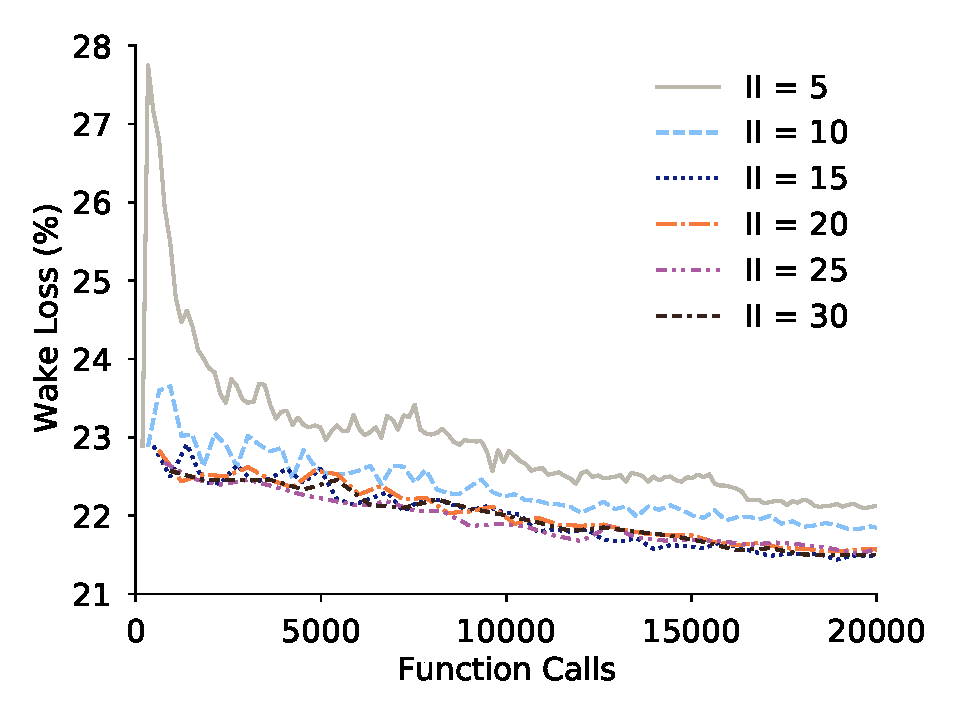
\includegraphics[width=\textwidth, trim={0cm 0cm 0cm 0cm}, clip]{tests/alpso_test_38turbs_36dirs.pdf}
		\caption{Comparing ALPSO convergence history for 38 turbines, 36 directions, and varying numbers of inner iterations.}
		\label{fig:alpso-ii-38-36}
	\end{minipage}\hspace{1pc}%
	\begin{minipage}[t]{0.48\textwidth}
		\centering
		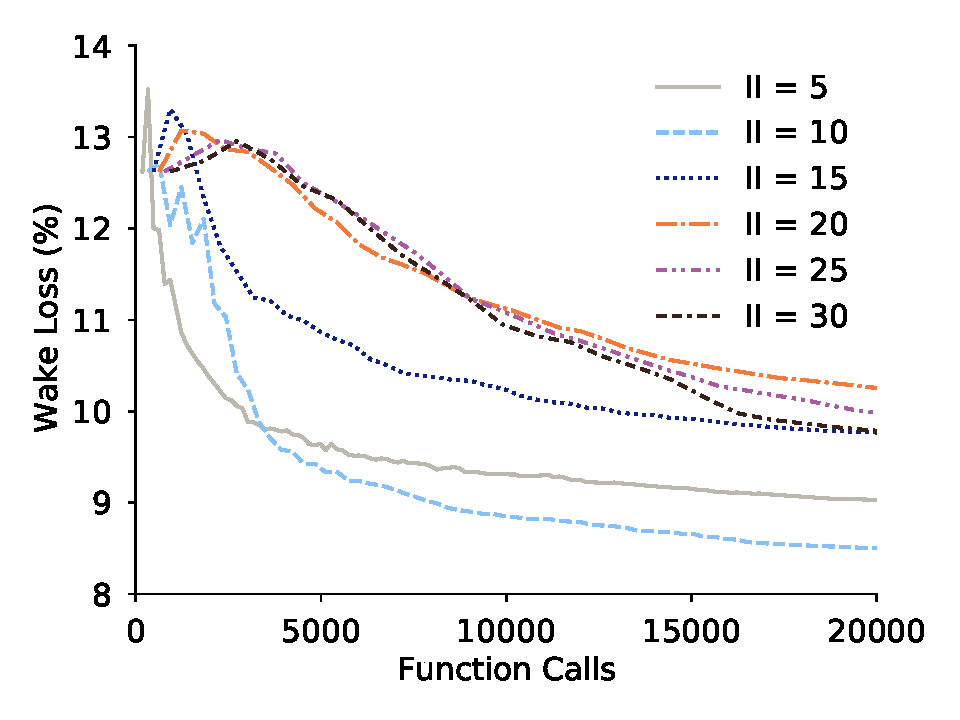
\includegraphics[width=\textwidth]{tests/alpso_test_60turbs_72dirs.pdf}
		\caption{Comparing ALPSO convergence history for 60 turbines, 72 directions, and varying numbers of inner iterations.}
		\label{fig:alpso-ii-60-72}
	\end{minipage} 
\end{figure}

While it may be noted that each optimization run with ALPSO is similar to running 30 optimizations using a gradient-based algorithm in population size, we decided to run a full set of 200 optimizations for each test, just as was done for SNOPT. This decision was to reflect how optimizations are often performed in practice, with many optimizations being run regardless of the algorithm being used. While ALPSO and other population-based algorithms do carry many samples of the design space concurrently, they are used to inform one another and drive to a single final solution, while the individual runs of gradient-based techniques are self-contained, do not influence one another, and represent a single solution. We consider a direct comparison between full optimizations, rather than population members, to be more informative in how results would look in practice using each algorithm. This approach also enables a direct comparison of function calls and the optimization objective.



\section{Applying WEC to the  Wake Models}
In this section we apply WEC, step by step, as presented in \cref{sec:dsrop} to the Bastankhah and Port\'e-Agel wake model and the Jensen cosine wake model. To test the wake spreading approaches discussed in \cref{sec:wecmethods}, we implemented each of them in the Bastankhah and Port\'{e}-Agel wake model. Once we understood which approach is most effective, we implemented and tested only that approach in the Jensen cosine model.

\subsection{Applying WEC to the Bastankhah and Port\'e-Agel Wake Model}


\subsubsection{Bastankhah and Port\'e-Agel WEC Step (1)}
The first parenthetical term of \cref{eq:bpa} defines the magnitude of the velocity deficit. The exponential terms determine the wake spread. The wake spread and velocity deficit are coupled through $\sigma_y$ and $\sigma_z$. However, because the spread and magnitude are expressed in separate terms, it is possible to adjust one without impacting the other. 

\subsubsection{Bastankhah and Port\'e-Agel WEC Step (2) - WEC-A}
 To gain direct control of wake spreading angle, we arranged the equations in such a way that the user specifies the wake spreading angle, rather than using a multiple of the default angle. 

To gain direct control of the wake spreading angle, we calculate the wake spreading slope that would correspond to the desired spreading angle ($\theta_\xi$) as
%
\begin{equation}
k_{y_{\xi}} = \tan{\theta_\xi}
\end{equation}
%
To get a final version, where a user can specify a desired spreading angle, we compare this against the original formula for $k_{y_{NEAR}}$ to obtain
%
\begin{equation}
k_{y_{\xi}} = \max(\tan{\theta_\xi}, k_{y_{NEAR}})
\end{equation}
%
We then use $k_{y_{\xi}}$ to re-define the wake spread at the point of far wake onset, $\sigma_{yo_{\xi}}$, as shown in \cref{eq:sigmay0xi}.
%
\begin{equation}\label{eq:sigmay0xi}
\sigma_{yo_{\xi}} = k_{y_{\xi}}x_o+\sigma_{yd}
\end{equation}
%
The definition for $\sigma_{yo_{\xi}}$ allows us to define the general form of the wake spread for all wake regions as shown in \cref{eq:sigmayxi}. 
%
\begin{equation}\label{eq:sigmayxi}
\sigma_{y_{\xi}} =
\begin{cases} k_y (x-x_o)+\sigma_{yo_{\xi}} & x >= x_o, k_y >= k_{y_{\xi}} \\
k_{y_{\xi}} (x-x_o)+\sigma_{yo_{\xi}} & x >= x_o, k_y < k_{y_{\xi}} \\
k_{y_{\xi}}x+\sigma_{yd} & x < x_o \\
\end{cases}
\end{equation}
%
The same process can also be applied to obtain $\sigma_{z_{\xi}}$. 

Now that we have direct control of the wake spreading angle, for angles greater than the default angle, we can apply the results directly to the exponential terms of \cref{eq:bpa} to obtain  a model that allows the user to specify a spreading angle without impacting the velocity deficit in the wake center as shown in \cref{eq:bpa_angle}.
\begin{equation}
\frac{\Delta \bar{u}}{\bar{u}_{\infty}} = \Bigg(1-\sqrt{1-\frac{C_T \cos{\gamma}}{8 \sigma_y \sigma_z/d^2}}~\Bigg) \exp{\bigg(-0.5\Big(\frac{y-\delta}{\sigma_{y_{\xi}}}\Big)^2\bigg)}\exp{\bigg(-0.5\Big(\frac{z-z_h}{\sigma_{z_{\xi}}}\Big)^2\bigg)}
\label{eq:bpa_angle}
\end{equation}
%
For WEC-A, The impact of $\theta_\xi$ is much more pronounced for turbines that are further upstream due to the increased wake growth rate. 

\subsubsection{Bastankhah and Port\'e-Agel WEC Step (2) - WEC-D}
In the diameter spreading method (WEC-D), independent control of the wake diameter is obtained by applying a factor, $\xi$, to $\sigma_y$ and $\sigma_z$ inside the exponential terms of \cref{eq:bpa}, as shown in \cref{eq:bpa_relax}.
% \begin{equation}
% 	\frac{\Delta U}{U_{\infty}} = \Bigg(1-\sqrt{1-\frac{C_T}{8\sigma^2/d_0^2}}~\Bigg) \exp{\Bigg(-\frac{1}{2}\bigg(\frac{z-z_h}{\xi\sigma}\bigg)^2\Bigg)}\exp{\Bigg(-\frac{1}{2}\bigg(\frac{y-\delta}{\xi\sigma}\bigg)^2\Bigg)}
% 	 \label{eq:bpa_relax}
% \end{equation}
\begin{equation}
\frac{\Delta \bar{u}}{\bar{u}_{\infty}} = \Bigg(1-\sqrt{1-\frac{C_T \cos{\gamma}}{8 \sigma_y \sigma_z/d^2}}~\Bigg) \exp{\bigg(-0.5\Big(\frac{y-\delta}{\xi \sigma_y}\Big)^2\bigg)}\exp{\bigg(-0.5\Big(\frac{z-z_h}{\xi \sigma_z}\Big)^2\bigg)}
\label{eq:bpa_relax}
\end{equation}
By increasing the value of $\xi$ we can widen the wakes without changing the magnitude of the velocity deficit in the center of the wakes. As the wakes widen, they mix and smooth out the local optima, as shown in \cref{fig:smoothing_bpa_wec_d}. 

\subsubsection{Bastankhah and Port\'e-Agel WEC Step (2) - WEC-H}

The third approach, WEC-H, is a sort of hybrid of the other two approaches of widening the wake. The wake diameter is multiplied in the far wake, but the near wake expands linearly until the pre-selected point where the wake diameter multiplier is applied. The basic theory for applying WECH to the Bastankhah and Port\'{e}-Agel model is shown in \cref{eq:sig0,eq:sig0wech,eq:sigywech}. The first step, \cref{eq:sig0}, is based on the original wake diameter calculation as shown in \cref{eq:sigmay}.
%
\begin{equation}\label{eq:sig0}
\sigma_{yo} = d\frac{\cos(\gamma)}{\sqrt(8)}
\end{equation}
%
\begin{equation}\label{eq:sig0wech}
\sigma_{yo,\xi} = \xi \sigma_{yo}
\end{equation}
%
\begin{align}\label{eq:sigywech}
\sigma_{y,\xi} = &
\begin{cases}
\xi (k_y (x-x_0) + d \frac{\cos(\gamma)}{\sqrt(8)}) & x > x_0 \\
\sigma_0 + x \frac{\sigma_{y0,\xi}-\sigma_0}{x_0} & x \le x_0 \\
\end{cases}
\end{align}
%
Where $\sigma_{yo}$ is the original wake spread at $x_0$, the onset of the far wake, $\sigma_{yo,\xi}$ is the wake spread at the onset of far wake after the application of the expansion factor, and $\sigma_{y,\xi}$ is the horizontal wake standard deviation to be used in the exponential terms of the Bastankhah and Port\'{e}-Agel model as shown in \cref{eq:wechapplied}. A similar approach can be used to fine $\sigma_{z,\xi}$.

\begin{equation}
\frac{\Delta \bar{u}}{\bar{u}_{\infty}} = \Bigg(1-\sqrt{1-\frac{C_T \cos{\gamma}}{8 \sigma_y \sigma_z/d^2}}~\Bigg) \exp{\bigg(-0.5\Big(\frac{y-\delta}{ \sigma_{y,\xi}}\Big)^2\bigg)}\exp{\bigg(-0.5\Big(\frac{z-z_h}{ \sigma_{z,\xi}}\Big)^2\bigg)}
\label{eq:wechapplied}
\end{equation}

Note that the $\sigma_{y,\xi}$ term is only applied to the wake width terms and the original model values are used in calculating the magnitude of the center-line wake deficit. As in WEC-A and WEC-D, increasing the value of the WEC factor, $\xi$, allows us to widen the wake without changing the magnitude of the velocity deficit in the center of the wake. As the wakes widen, they mix and smooth out the local optima. 


\begin{figure}[ht]
	\centering
	\begin{minipage}[t]{0.47\textwidth}
		\centering
		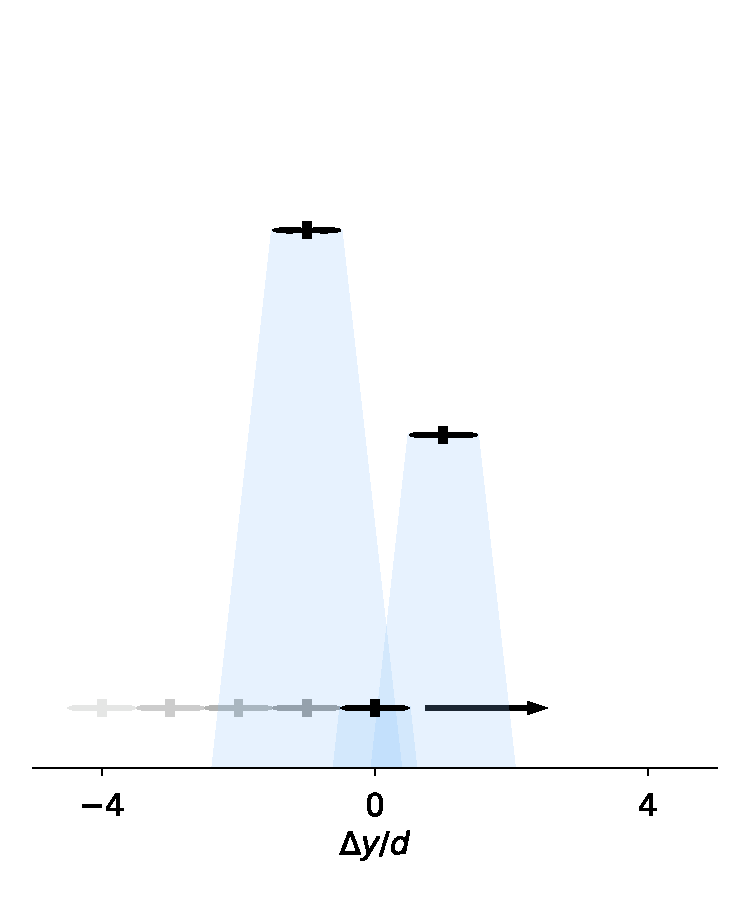
\includegraphics[width=\textwidth, trim={-2.0cm -0.0cm -2.0cm 3.5cm}, clip]{final_images/layouts/3turb-design-space}
		\caption{Simple wind farm, seen from above, used to demonstrate the effects of the WEC factors, $\theta_\xi$ and $\xi$, on the wind farm layout design space (see \cref{fig:smoothing_bpa_wec_d}). Wind is from the top.}
		\label{fig:smoothing_locations_bpa}
	\end{minipage}\hspace{1pc}
	%
%	\begin{minipage}[t]{0.47\textwidth}
%		\centering
%		\includegraphics[width=\textwidth]{smoothing_bpa_wec_a}
%		\caption{The impact of changing the wake spread angle, $\theta_\xi$, for WEC-A on a simple wind farm layout design space with one movable turbine and one wind direction (see \cref{fig:smoothing_locations_bpa}) using the Bastankhah and Port\'{e}-Agel wake model. The local optimum between the wakes disappears as the WEC factor increases.}
%		\label{fig:smoothing_bpa_wec_a}
%	\end{minipage} 
	%
	\begin{minipage}[t]{0.47\textwidth}
		\centering
		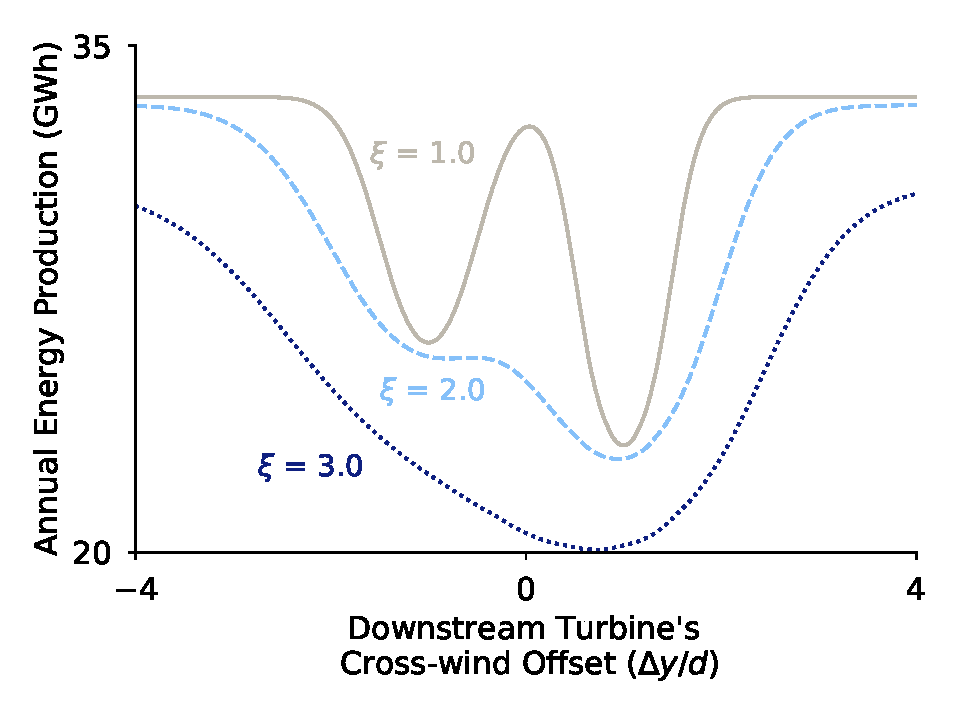
\includegraphics[width=\textwidth]{smoothing_bpa_wec_d}
		\caption{The impact of the relaxation factor, $\xi$, for WEC-D on a simple wind farm layout design space with one movable turbine and one wind direction (see \cref{fig:smoothing_locations_bpa}) using the Bastankhah and Port\'{e}-Agel wake model. The local optimum between the wakes disappears as the WEC factor increases.}
		\label{fig:smoothing_bpa_wec_d}
	\end{minipage} %\hspace{1pc}
	%
%	\begin{minipage}[t]{0.47\textwidth}
%		\centering
%		\includegraphics[width=\textwidth]{smoothing_bpa_wec_h}
%		\caption{The impact of changing the wake spread angle, $\xi$, for WEC-H on a simple wind farm layout design space with one movable turbine and one wind direction (see \cref{fig:smoothing_locations_bpa}) using the Bastankhah and Port\'{e}-Agel wake model. The local optimum between the wakes disappears as the WEC factor increases.}
%		\label{fig:smoothing_bpa_wec_h}
%	\end{minipage}
\end{figure}

\subsubsection{Bastankhah and Port\'e-Agel WEC Step (3)}
To gain the benefits of WEC without losing the accuracy of the wake model, the optimization must be run multiple times, in a continuation approach, with values of $\xi$ or $\theta_\xi$ decreasing to 1 or 0 respectively. The results from optimizing with each value of $\xi$ or $\theta_\xi$ can then be used to warm start the next optimization. In this way, the gradient-based optimization can intelligently explore the design space and then refine the model to find a final, more accurate, result. The iterative optimizations are generally fairly fast due to starting from the previous optimized solution. In the following section we will show how we determined which WEC method to use and the corresponding values of $\xi$ or $\theta_\xi$ to use in practice.

\subsection{Comparing the WEC methods as applied to the Bastankhah and Port\'e-Agel wake model}\label{sec:bpa_wec_comparison}

Once WEC-A, WEC-D, and WEC-H were implemented in the Bastankhah and Port\'{e}-Agel model, we compared the performance of each method by varying both the number of intermediate optimizations, or steps, to run and the maximum values of the WEC factor, $\xi$ or $\theta_\xi$, to use. To investigate the WEC methods and parameter selection, we used 200 different starting layouts for a wind farm problem with 38 turbines and 12 wind directions with a constant wind speed of 8 m/s in all directions as shown in \cref{fig:method_study_layout,fig:nantucket12dirs}. 

\begin{figure}[h!]
	\centering
	\begin{minipage}[t]{18pc}
		\centering
		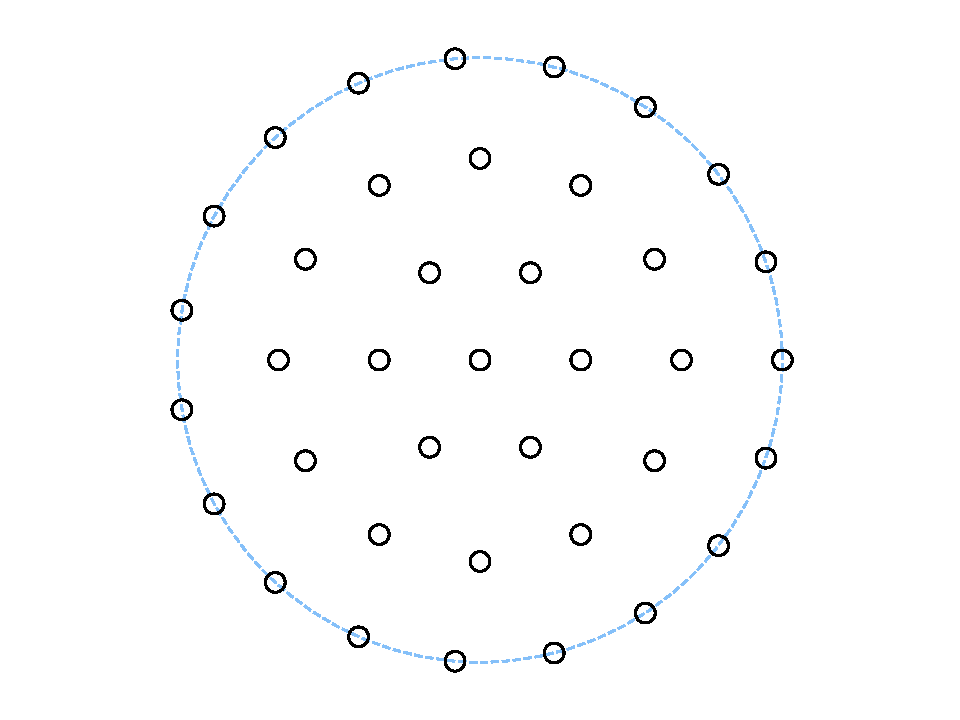
\includegraphics[width=\textwidth, trim={1.5cm, 0cm, 2.0cm, 0cm}, clip]{final_images/layouts/38_turb_start.pdf}
		\caption{Baseline layout for the WEC method comparison study. Turbine circles are to scale. The dashed blue line represents the wind farm boundary constraint.}
		\label{fig:method_study_layout}
	\end{minipage}\hspace{1pc}%
	\begin{minipage}[t]{18pc}
		\centering
		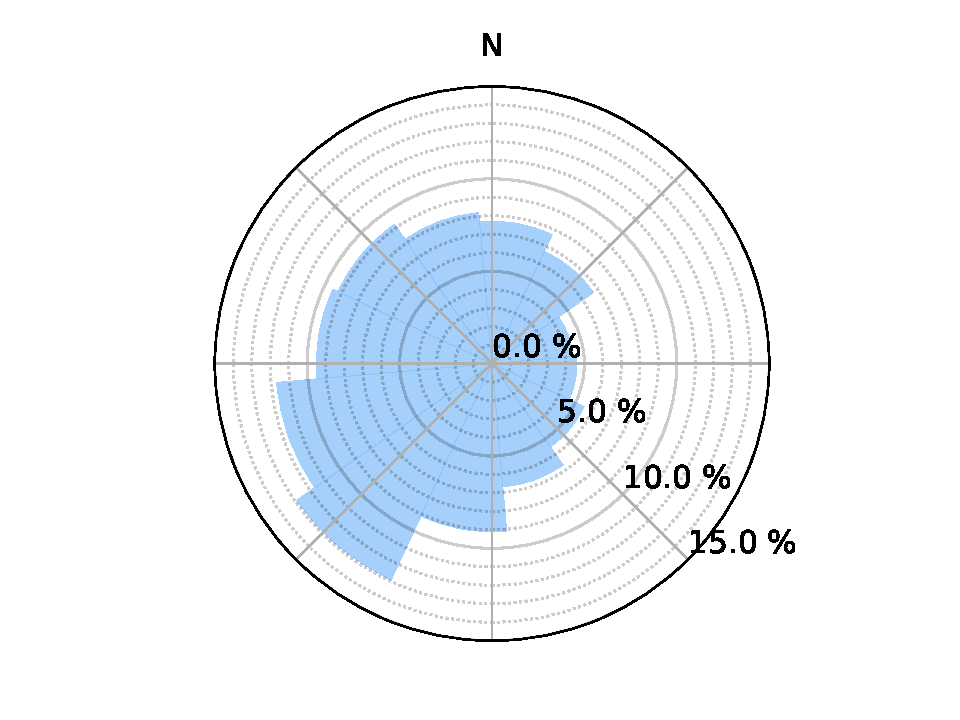
\includegraphics[width=\textwidth, trim={2.0cm 0cm 1.5cm 0cm}, clip]{final_images/windroses/freqwindrose_12_dir.pdf}
		\caption{Directional probability wind rose for the WEC method comparison study. This is the Nantucket wind rose binned into 12 directions \cite{wrcc2017}. For the WEC method study, we used a constant wind speed of 8 m/s.}
		\label{fig:nantucket12dirs}
	\end{minipage} 
\end{figure}


When the maximum WEC factor value was varied, the number of steps was held at six. When the number of steps was varied, the maximum WEC factor was held at $\theta_\xi = 9 ^\circ$, $\xi=3$, and $\xi=3$, for WEC-A, WEC-D, and WEC-H respectively. All 200 starting layouts were tested with each parameter set while solving the optimization problem shown in \cref{eq:obj_wec_methods}. 
%
\begin{equation}
\label{eq:obj_wec_methods}
\begin{aligned} [b]
\underset{x_i,y_i}{\textrm{maximize}} \quad & AEP(x_i,y_i,)~~i=1...38\\
\textrm{subject to} \quad & s_{i,j} \geq 2\*d~~i,j=1...38~~i \neq j\\
& [x_c-x_i]^2+[y_c-y_i]^2 \leq r_{b}^2~~i=1...38
\end{aligned}
\end{equation}
%
In \cref{eq:obj_wec_methods}, $(x_i,y_i)$ is the position of each turbine $i$, $s_{i,j}$ represents the separation distance between each pair of turbines $i$ and $j$, $(x_c,y_c)$ is the location of the center of the wind farm, and $r_b$ is the radius of the wind farm boundary. For the case here used to compare WEC methods, the $k*$ value was not adjusted to the local turbulence intensity during optimization, but was adjusted for calculating the results shown. This case has a total of 76 variables and 741 constraints.

When the optimizations for all starting layouts and parameter combinations were complete, we compared the minimum, mean, and standard deviation of wake loss (energy lost due to wake effects) across all the optimizations. Wake loss percentage was calculated as shown in \cref{eq:wake_loss}.
%
\begin{equation} \label{eq:wake_loss}
	L = 100 \bigg( 1 - \frac{AEP_0}{AEP_t} \bigg)
\end{equation}
%
 In \cref{eq:wake_loss}, $AEP_0$ represents the optimized AEP found from a given starting layout and $AEP_t$ is the theoretical maximum AEP calculated as shown in \cref{eq:aept}. 
 %
 \begin{equation} \label{eq:aept}
 AEP_t = (24)(365)\sum_{j=1}^{n_d} \bigg( p_j P \bigg)  
 \end{equation}
 %
 In \cref{eq:aept}, $P$ is the power of a single un-waked wind turbine calculated using \cref{eq:power}. 
 
% The minimum wake loss results are shown in \cref{fig:aepmin-wm,fig:aepmin-ws}.
%%
%\begin{figure}[ht]
%	\centering
%	\begin{minipage}[t]{0.47\textwidth}
%		\centering
%		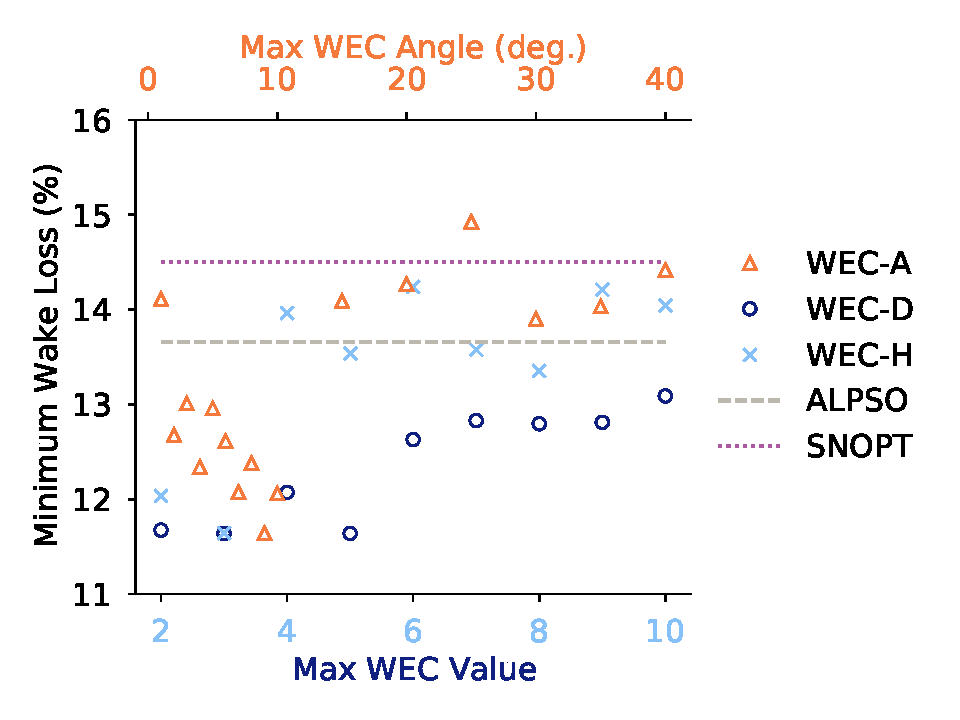
\includegraphics[width=\textwidth, trim={0cm 0cm 0cm 0cm}, clip]{maxwec_const_nsteps6_min}
%		\caption{Minimum wake loss results for varying the maximum WEC expansion parameter while hold the number of steps constant at six. Each data point represents 200 separate optimizations with different starting points.}
%		\label{fig:aepmin-wm}
%	\end{minipage}\hspace{1pc}
%	% Figure displaying results from aep vs crosswind position tests for Jensen
%	\begin{minipage}[t]{0.47\textwidth}
%		\centering
%		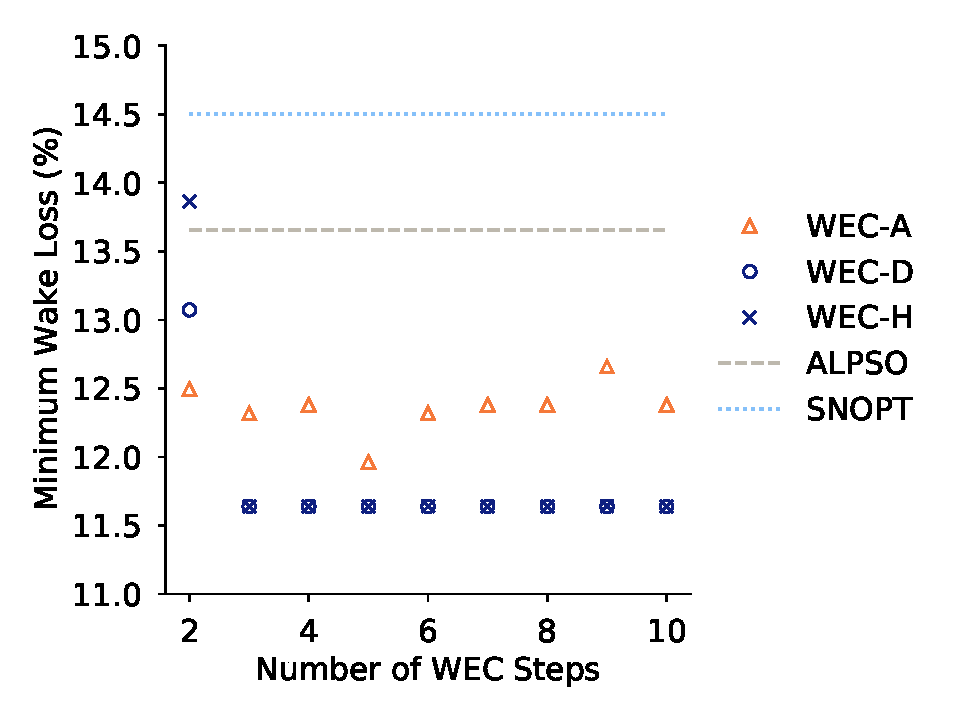
\includegraphics[width=\textwidth]{nsteps_const_maxwec_min}
%		\caption{Minimum wake loss results for varying the number of WEC steps while holding the expansion parameter constant at three. Each data point represents 200 separate optimizations with different starting points.}
%		\label{fig:aepmin-ws}
%	\end{minipage}
%\end{figure}
%
We found that the minimum wake loss is achieved when the maximum WEC angle is $9^\circ$ for WEC-A and when the maximum WEC value is 3 for WEC-D and WEC-H. While WEC generally out performs SNOPT alone, lower WEC values tend to result in less wake loss. There does not appear to be a clear relationship between minimum wake loss and number of steps for WEC-A. WEC step numbers greater than or equal to 3 achieve approximately equal minimum wake loss for WEC-D and WEC-H, but on average WEC-D performs much better.

The mean wake loss results are provided in \cref{fig:aepmean-wm,fig:aepmean-ws}. Here we see that, on average, WEC-D results in less wake loss with a WEC value of 3 and using 5 or more steps, while WEC-A has its lowest average wake loss for a maximum WEC angle of $6^\circ$, and WEC-H minimizes average wake loss most with lower WEC values. On average, wake loss minimized using WEC-A or WEC-H does not appear to be impacted by changing the number of steps.

\begin{figure}[ht]
	\centering
	\begin{minipage}[t]{0.47\textwidth}
		\centering
		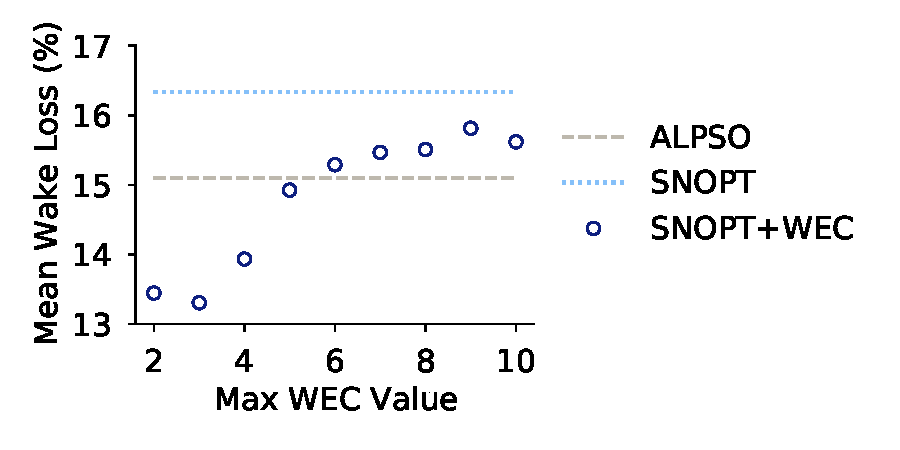
\includegraphics[width=\textwidth, trim={0cm 0cm 0cm 0cm}, clip]{tests/maxwec_const_nsteps6_mean}
		\caption{Mean wake loss results for varying the maximum WEC expansion parameter while holding the number of steps constant at six. Each data point represents 200 separate optimizations with different starting points. Note: the WEC value and WEC angle axes are not directly comparable.}
		\label{fig:aepmean-wm}
	\end{minipage}\hspace{1pc}
	% Figure displaying results from aep vs crosswind position tests for Jensen
	\begin{minipage}[t]{0.47\textwidth}
		\centering
		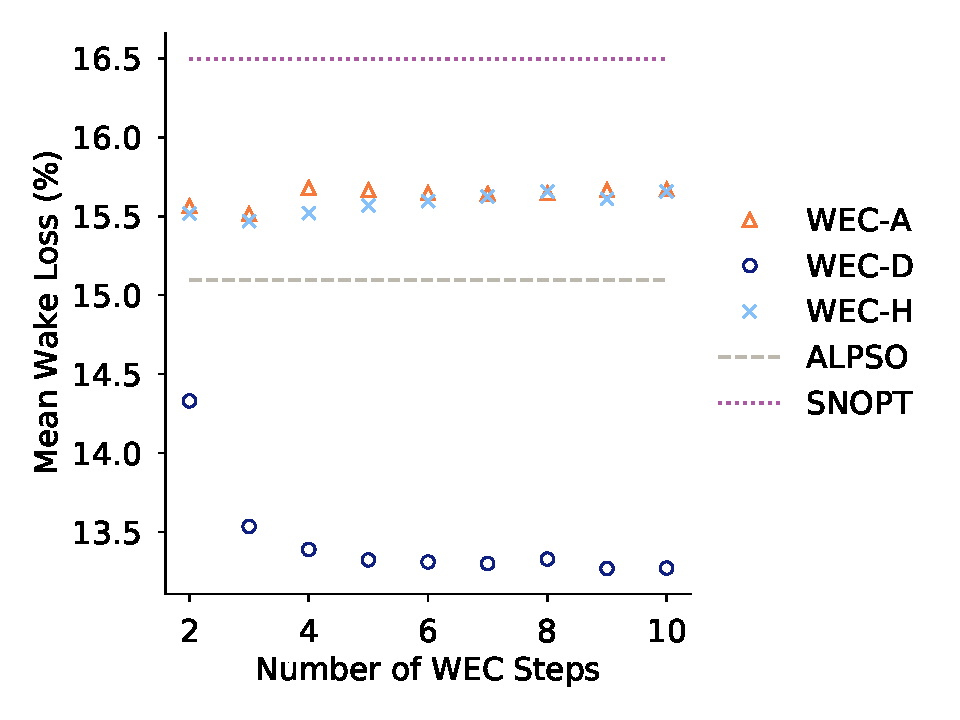
\includegraphics[width=\textwidth]{tests/nsteps_const_maxwec_mean}
		\caption{Mean wake loss results for varying the number of WEC steps while holding the expansion parameter constant at three. Each data point represents 200 separate optimizations with different starting points.}
		\label{fig:aepmean-ws}
	\end{minipage}
\end{figure}

The lowest standard deviations occur when the WEC angle is $5^\circ$ for WEC-A, the WEC value is 3 for WEC-D, and when the WEC value is 2 for WEC-H. There is no clear relationship between number of steps and the standard deviation for WEC-A and WEC-H, but we found it best to use at least 4 or 5 steps with WEC-D to achieve a small standard deviation (meaning more consistent results).

%\begin{figure}[ht]
%	\centering
%	\begin{minipage}[t]{0.47\textwidth}
%		\centering
%		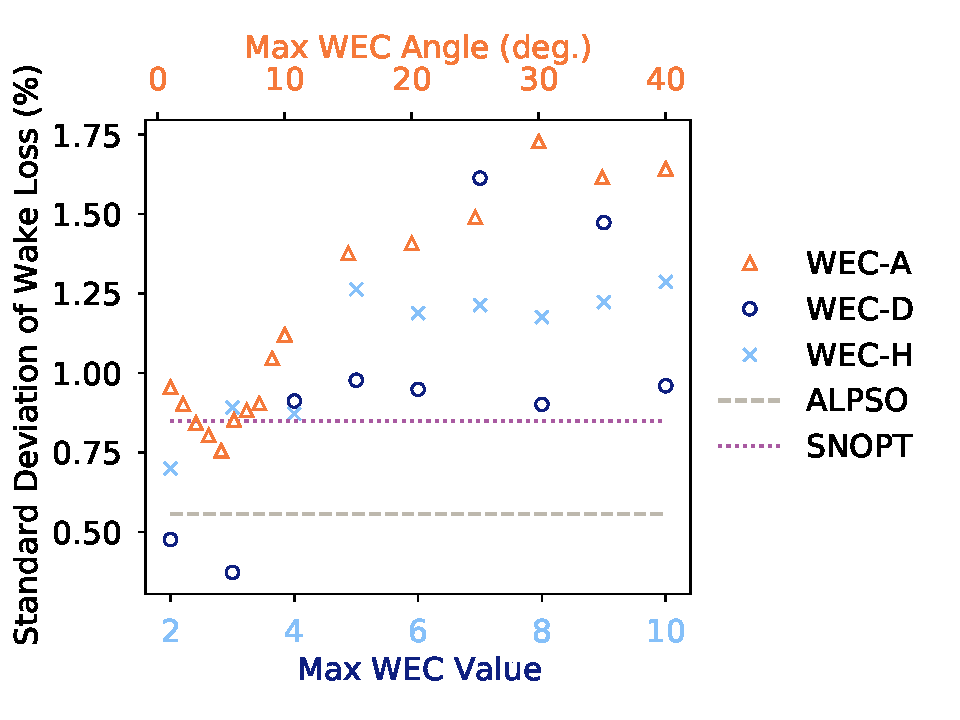
\includegraphics[width=\textwidth, trim={0cm 0cm 0cm 0cm}, clip]{maxwec_const_nsteps6_std}
%		\caption{Standard deviation of wake loss results for varying the maximum WEC expansion parameter while holding the number of steps constant at six. Each data point represents 200 separate optimizations with different starting points.}
%		\label{fig:aepstd-wm}
%	\end{minipage}\hspace{1pc}
%	% Figure displaying results from aep vs crosswind position tests for Jensen
%	\begin{minipage}[t]{0.47\textwidth}
%		\centering
%		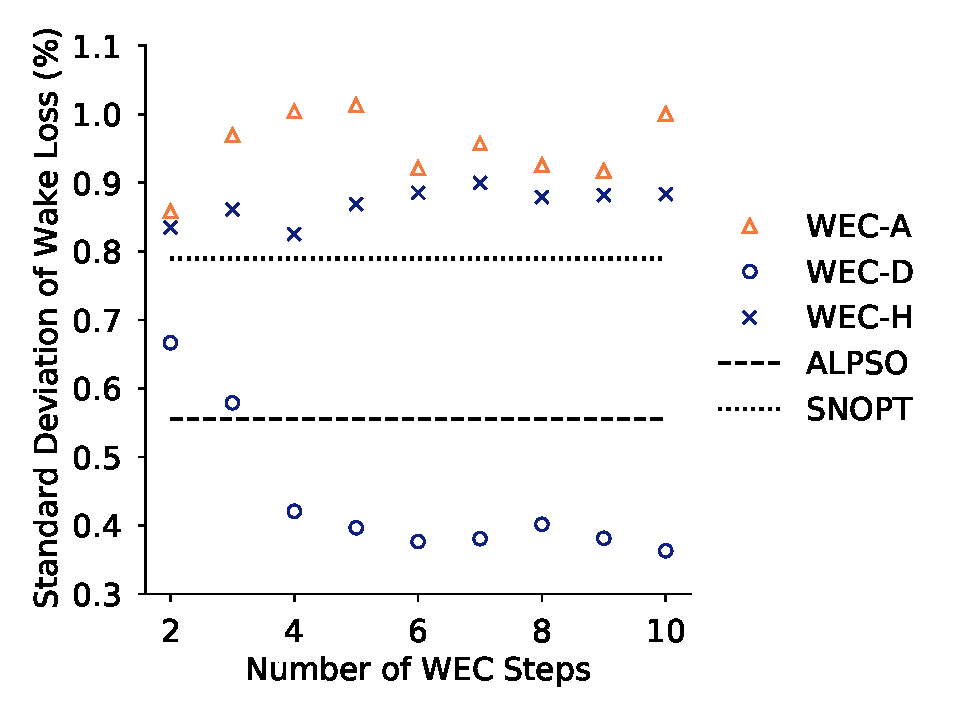
\includegraphics[width=\textwidth]{nsteps_const_maxwec_std}
%		\caption{Standard deviation of wake loss results for varying the number of WEC steps while holding the expansion parameter constant at three. Each data point represents 200 separate optimizations with different starting points.}
%		\label{fig:aepstd-ws}
%	\end{minipage}
%\end{figure}

 As discussed, we found that the WEC-D method is the best wake spreading method we investigated as it had the lowest minimum, mean, and standard deviation of wake loss. We decided to use WEC-D with 6 steps and a maximum WEC spread parameter of three for the remaining studies.
 
 The better performance of WEC-D over WEC-A and WEC-H can be explained by the fact that both WEC-A and WEC-H alter the wake shape, while WEC-D only multiplies the standard deviation of the basis functions in a manner consistent with Gaussian continuation optimization theory as discussed in \cite{mobahi2015}. In the balance of this paper we will refer to WEC-D as WEC because the other methods have no more relevance in this discussion. 
 
\subsection{Applying WEC to the Jensen Cosine Wake Model}
In this section we apply WEC, step by step as presented in \cref{sec:dsrop}, to the Jensen Cosine wake model. A diagram displaying the Jensen cosine wake model from an overhead perspective is shown in  \cref{fig:JensenDiagrams}. This diagram will give context to the variables and parameters discussed in this section.

\subsubsection{Jensen Cosine WEC Step (1)} 
%Identify where the magnitude and spread of the wake are within the Jensen Cosine equation.

The cosine factor, $f_\theta$, in \cref{eq:JensenVelocityDeficit} controls the wake spread for the Jensen Cosine wake model. By breaking down the cosine factor into its constituent parameters, it is possible to adjust the wake spread without impacting the velocity deficit in the center of the wake.

As can be seen in \cref{eq:JensenCosineAdjustment}, $f_\theta$ is a function of $\theta$, which represents the angle between the wake's center line and the downwind turbine's location as measured from the wake vertex (a distance $z$ along the wake center line upstream of the wind turbine). This angle $\theta$ can be determined using \cref{eq:Theta}.

% Equation for calculating theta, the angle between the wake's vertex and the point of interest
\begin{equation}
\theta = \tan^{-1}\Big( \frac{\Delta y}{\Delta x + z} \Big)
\label{eq:Theta}
\end{equation}

In \cref{eq:Theta}, $\Delta x$ and $\Delta y$ represent the downwind and crosswind spacing between the upwind turbine and the downwind location of interest. The variable $z$ represents the distance between the wake's vertex and the upwind turbine. By adjusting the value of $z$, we are able to increase or decrease the wake's spread. An expression for $z$ based on the initial wake diameter can be found below in \cref{eq:vertexdistance}.

\begin{equation}
z = \frac{r_0}{tan(\beta)}
\label{eq:vertexdistance}
\end{equation} 


\subsubsection{Jensen Cosine WEC Step (2)}
We can directly adjust the wake spread without impacting the magnitude of the deficit in the center of the wake by applying a relaxation factor, $\xi$, to the rotor radius, $r_0$, in \cref{eq:vertexdistance}, as seen below in \cref{eq:WECvertexcistance}.

\begin{equation}
z = \frac{\xi r_0}{tan(\beta)}
\label{eq:WECvertexcistance}
\end{equation}

Through a series of substitutions, this new vertex distance, \cref{eq:WECvertexcistance}, may be combined with the Jensen cosine wake model to obtain \cref{eq:JensenVelocityDeficitCombined}.

% Insert equation: final equation displaying the direct relationship between the velocity deficit and the relaxation factor, xi.
\begin{equation}
\frac{\Delta \bar{u}}{\bar{u}_\infty} = 1 - 2a \Bigg[  \bigg(\frac{r_0}{r_0 + \alpha x} \bigg) \Bigg]^2 \frac{1}{2} \Bigg(1 + cos\Bigg[\frac{\pi}{\beta} tan^{-1}\Bigg(\frac{\Delta y}{\Delta x + \frac{\xi r_0}{tan(\beta)}} \Bigg) \Bigg] \Bigg)
\label{eq:JensenVelocityDeficitCombined}
\end{equation}

Because we have inserted the relaxation factor, $\xi$, into \cref{eq:JensenVelocityDeficitCombined}, we may adjust the wake spread without changing the velocity deficit in the center of the wake. Note that this is true because when $\Delta y = 0$, the term inside the inverse tangent in \cref{eq:JensenVelocityDeficitCombined} goes to zero, regardless of the value of $\xi$. Because this is the only place where the relaxation factor is found in \cref{eq:JensenVelocityDeficitCombined}, this means that the velocity deficit will be constant with respect to $\xi$ at the wake center. This behavior is shown in \cref{fig:smoothing_locations_jensen,fig:smoothing_jensen_wec_d}, which also shows that local optima can be smoothed out through WEC for the Jensen Cosine model.

% Figure describing setup for aep vs crosswind position tests for Jensen
\begin{figure}[ht]
	\centering
	\begin{minipage}[t]{0.43\textwidth}
		\centering
		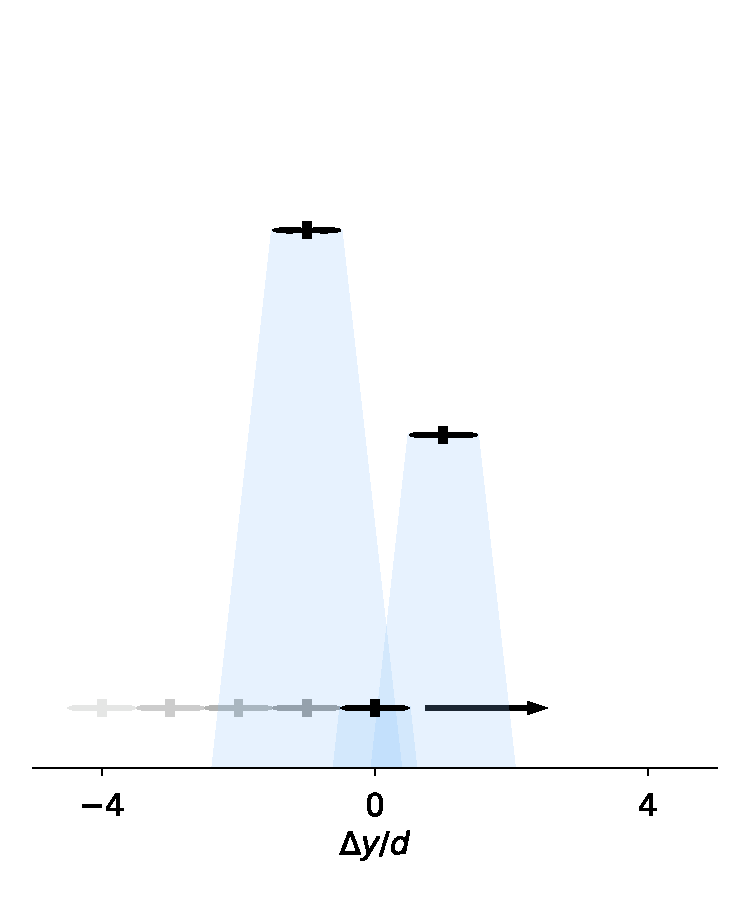
\includegraphics[width=\textwidth, trim={-0.5cm -0.5cm -0.5cm 3.25cm}, clip]{final_images/layouts/3turb-design-space}
		\caption{Simple wind farm, seen from above, used to demonstrate the effects of the WEC factor $\xi$, on the wind farm layout design space (see \cref{fig:smoothing_jensen_wec_d}). Wind is from the top.}
		\label{fig:smoothing_locations_jensen}
	\end{minipage}\hspace{1pc}
	% Figure displaying results from aep vs crosswind position tests for Jensen
	\begin{minipage}[t]{0.52\textwidth}
		\centering
		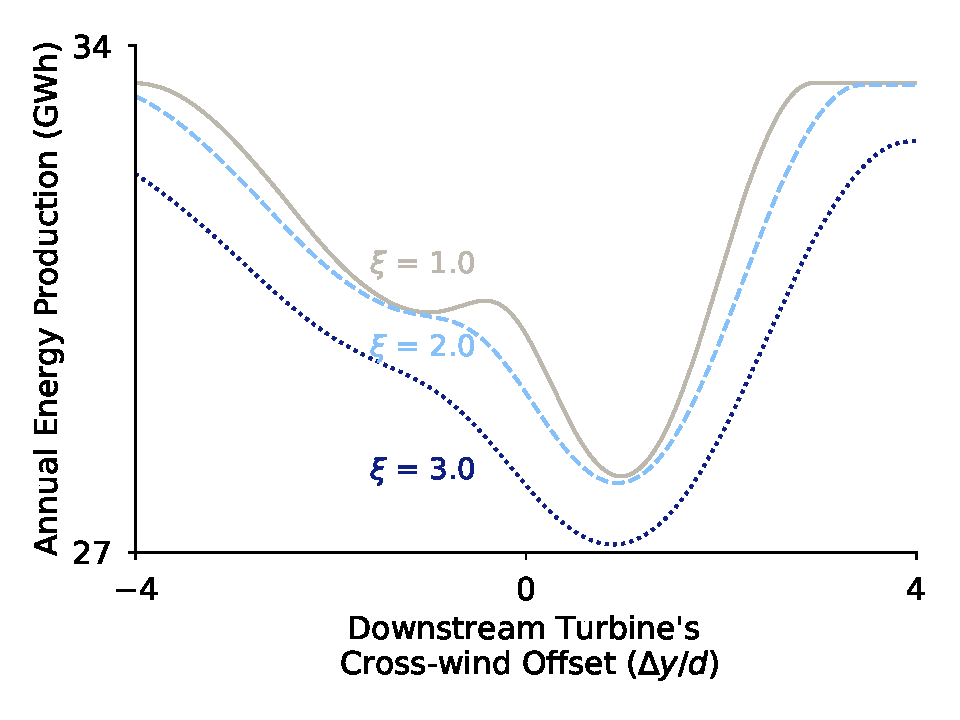
\includegraphics[width=\textwidth]{smoothing_jensen_wec_d}
		\caption{The impact of changing the wake spread angle, $\xi$, for WEC on a simple wind farm layout design space with one movable turbine and one wind direction (see \cref{fig:smoothing_locations_jensen}) using the Jensen cosine wake model. The local optimum between the wakes disappears as the WEC factor increases.}
		\label{fig:smoothing_jensen_wec_d}
	\end{minipage}
\end{figure}

\subsubsection{Jensen Cosine WEC Step (3)}

The final step of the WEC method is the same for all models, with the exception that different WEC factors and number of WEC steps may be optimal for different wake models.

\subsection{Testing WEC with the Jensen Cosine Wake Model}
As a proof of concept in applying WEC to other wake models, we implemented WEC with the Jensen cosine model using the same maximum value of $\xi$ (three) and the same number of WEC steps (six) as found best for use with WEC as applied to the Bastankhah and Port\'{e}-Agel model in \cref{sec:bpa_wec_comparison}. We tested WEC using the Jensen cosine model applied to the case shown in \cref{fig:method_study_layout,fig:nantucket12dirs,eq:obj_wec_methods} using the same 200 starting layouts as used to test the various WEC methods. Results of this test, shown in \cref{fig:jensen-38-wake-loss,fig:jensen-38-wake-fcalls}, clearly demonstrate significant improvement in minimum, median, and standard deviation of wake loss for using WEC with SNOPT as opposed to using SNOPT alone, at the expense of an increase in the number of function calls.


\begin{figure}[h!]  
	\centering
	\begin{minipage}[t]{18pc}    
		\centering
		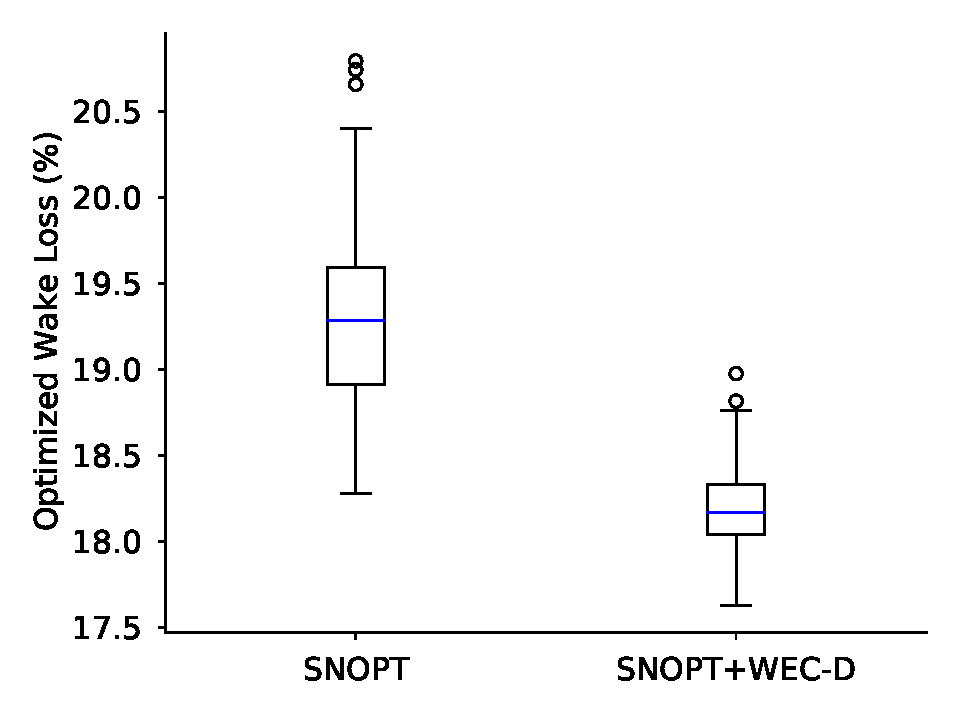
\includegraphics[width=\textwidth, trim={0cm 0cm 0cm 0cm}]{final_images/results/38turbs_results_jensen_percent_wake_loss.pdf}
		\caption{Wake loss percentage for 200 optimizations using the Jensen model with and without WEC. These optimizations were performed on the 38 turbine wind farm and 12 direction wind rose shown in \cref{fig:method_study_layout,fig:nantucket12dirs}.}
		\label{fig:jensen-38-wake-loss}
	\end{minipage}\hspace{1pc}
	\begin{minipage}[t]{18pc}    
		\centering
		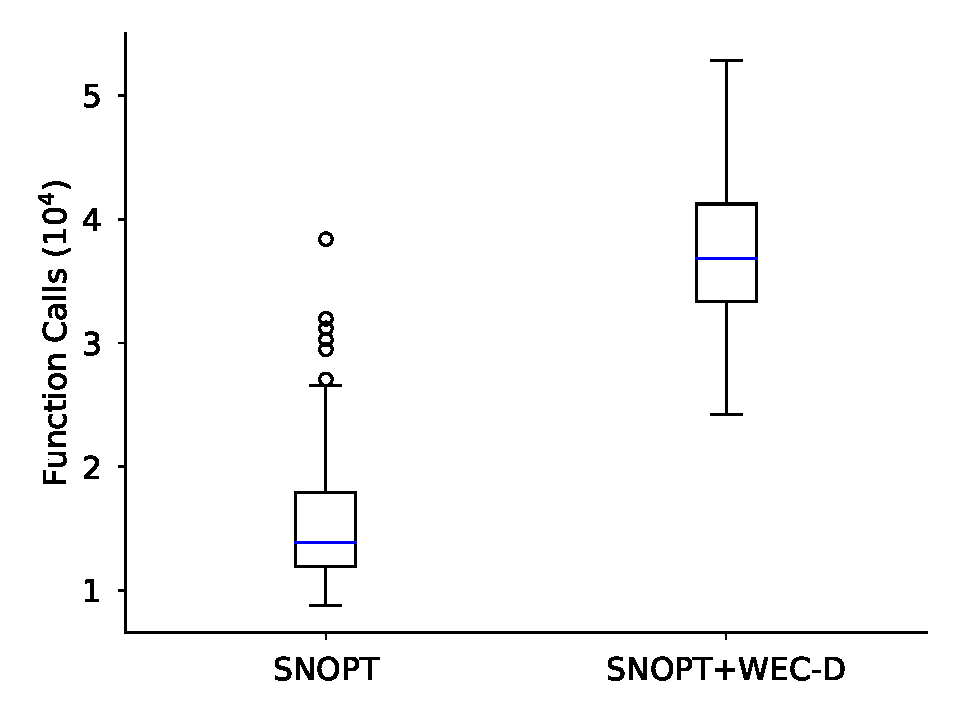
\includegraphics[width=\textwidth, trim={0cm 0cm 0cm 0cm}]{final_images/results/38turbs_results_jensen_fcalls.pdf}
		\caption{Function calls for 200 optimizations using the Jensen model with and without WEC-D. These optimizations were performed on the 38 turbine wind farm and 12 direction wind rose shown in \cref{fig:method_study_layout,fig:nantucket12dirs}.}
		\label{fig:jensen-38-wake-fcalls}
	\end{minipage}
\end{figure}

%\subsection{Testing WEC with ALPSO}
%
%Beside knowing if WEC works with different wake models, it is also of interest to know if WEC can improve the results of gradient-free algorithm. To test this we ran the same case shown in \cref{fig:round_case,fig:nantucket12dirs} using ALPSO with and without WEC. The results of this test are shown in \cref{
%
%\begin{figure}[h!]  
%	\centering
%	\begin{minipage}[t]{18pc}    
%		\centering
%		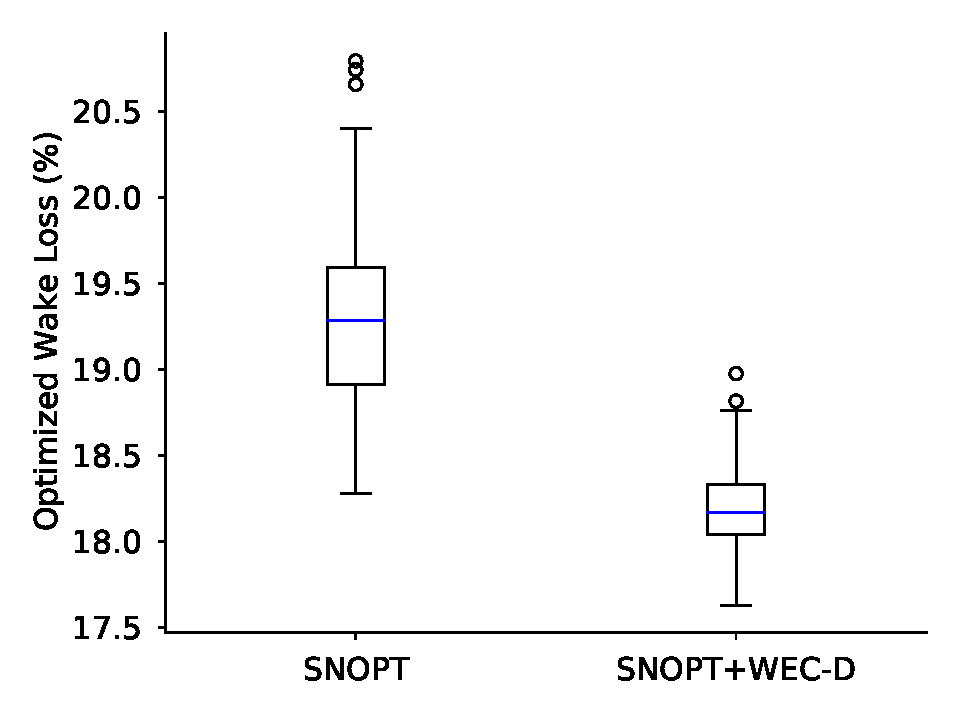
\includegraphics[width=\textwidth, trim={0cm 0cm 0cm 0cm}]{final_images/results/38turbs_results_jensen_percent_wake_loss.pdf}
%		\caption{Wake loss percentage for 200 optimizations using the Jensen model with and without WEC. These optimizations were performed on the 38 turbine wind farm and 12 direction wind rose shown in \cref{fig:method_study_layout,fig:nantucket12dirs}.}
%		\label{fig:jensen-38-wake-loss}
%	\end{minipage}\hspace{1pc}
%	\begin{minipage}[t]{18pc}    
%		\centering
%		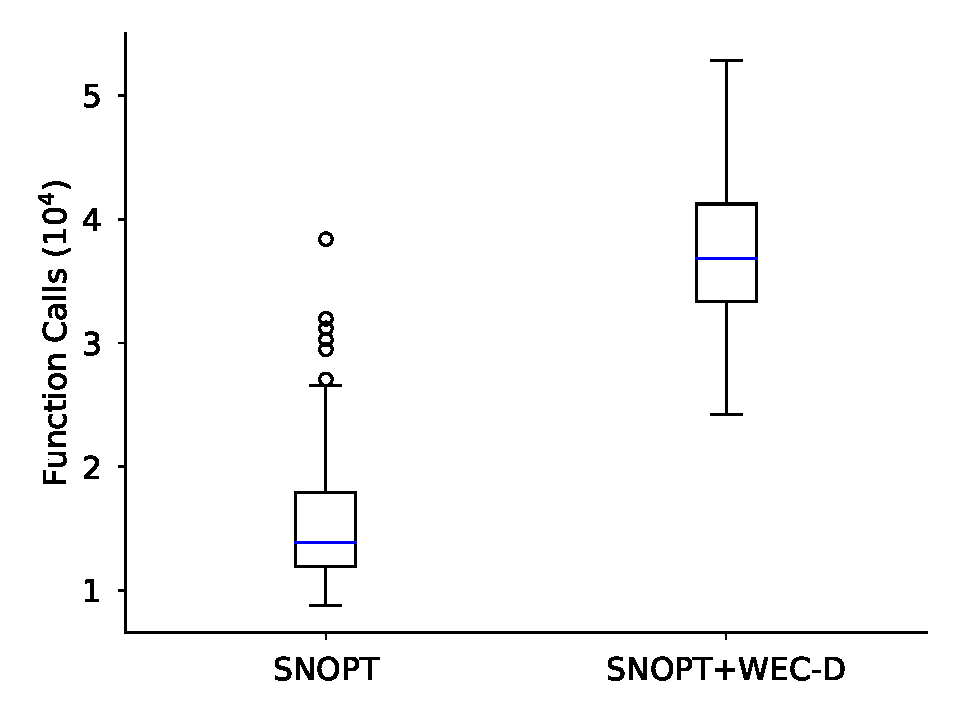
\includegraphics[width=\textwidth, trim={0cm 0cm 0cm 0cm}]{final_images/results/38turbs_results_jensen_fcalls.pdf}
%		\caption{Function calls for 200 optimizations using the Jensen model with and without WEC. These optimizations were performed on the 38 turbine wind farm and 12 direction wind rose shown in \cref{fig:method_study_layout,fig:nantucket12dirs}.}
%		\label{fig:jensen-38-wake-fcalls}
%	\end{minipage}
%\end{figure}

%\subsection{Applying WEC to the FLORIS Wake Model}
%In this section we apply WEC, step by step, as presented in \cref{sec:dsrop} to the FLORIS wake model.  
%
%%\todo{need to get better figure. remember to update caption once new figure inserted.}
%%\begin{figure}[h]
%%    \centering
%%    \includegraphics[width=0.3\linewidth]{FLORISDiagram1}
%%    \caption{Diagram displaying the three wake zones in the FLORIS turbine wake model. A higher quality diagram would have been constructed if there had been sufficient time. The black outer lines represent the outermost wake zone (mixing zone) which expands from the wind turbine as the air travels downstream. The blue lines represent the middle wake zone (far zone) which retains nearly the same width with distance from the turbine. Finally, the green lines represent the innermost wake zone (near wake) which converges to a point some distance from the turbine. The velocity deficit associated with each wake zone increases from the outermost wake zone to the innermost wake zone.}
%%    \label{fig:FLORISDiagram}
%%\end{figure}
%
%\subsubsection{FLORIS WEC Step (1)}
%%\textbf{Identify where the magnitude and spread of the wake are within the FLORISSE equation.}
%
%We began by determining where in the FLORIS wake model to apply the relaxation factor. Similar to the Jensen Cosine wake model, we decided to apply the relaxation factor to the original wake diameter in the FLORIS wake model. Because the increased wakes would result in larger wake overlaps, we decided that our implementation of WEC would need to occur before any area overlap calculations took place. Based on Figure 3 of Gebraad et. al's paper \cite{gebraad2014}, we decided that the most intuitive option would be to implement the relaxation factor in the wake diameter equation (\cref{eq:FLORISWakeWidth}).
%
%\begin{equation}
%    D_{w,i,q} = D_i + 2k_em_{e,q}(x - X_i)
%    \label{eq:FLORISWakeWidth}
%\end{equation}
%
%In \cref{eq:FLORISWakeWidth}, $D_{w,i,q}$ represents the diameter of the wake for the turbine of index $i$ within the wake-zone $q$, $D_i$ represents the rotor-diameter of turbine $i$, $k_e$ and $m_{e,q}$ represent wake expansion coefficients, $x$ represents the distance downwind from the wake-generating turbine to turbine $i$, and $X_i$ represents the x-coordinate of turbine $i$. In this equation, $k_e$ and $m_{e,q}$ determine the rate of expansion while $D_i$ represents an initial wake width.
%
%\subsubsection{FLORIS WEC Step (2)}
%%\textbf{Apply relaxation factor to the FLORIS equation. Show the aep vs crosswind position plot to demonstrate the velocity deficit is unchanged in the center of the wake and that the wakes are capable of being spread out. Briefly describe this plot and how the wec factor affects it.}
%
%If we applied the relaxation factor to $k_e$ or $m_{e,q}$ in \cref{eq:FLORISWakeWidth}, the rate of wake expansion would be affected, which violates the conditions for WEC described at the start of the Methods section. On the other hand, applying the relaxation factor to $D_i$ would expand the wake without affecting the rate of wake expansion. Therefore, we decided to apply the relaxation factor to $D_i$ in \cref{eq:FLORISWakeWidth} to obtain \cref{eq:FLORISWECWakeWidth}.
%
%\begin{equation}
%    D_{w,i,q}' = D_i' + 2k_em_{e,q}(x - X_i)
%    \label{eq:FLORISWECWakeWidth}
%\end{equation}
%
%Where $D_{w,i,q}'$ represents the adjusted wake width from applying WEC and $D_i'$ represents the adjusted initial wake diameter from applying WEC. We applied a relaxation factor to all wake zones within the FLORIS wake model. The resulting equations controlling the wake diameters for various wake zones in the FLORIS model are displayed below in \cref{eq:FLORISWECWakeDiameterPiecewise}. In this equation, $q$ represents the wake zone being used (i.e., $q = 1$ for the innermost wake zone, $q = 2$ for the middle wake zone, and $q = 3$ for the outermost wake zone).
%
%%\begin{equation}
%%    D_i' = \xi D_i
%%    \label{eq:FLORISWECWakeDiameter}
%%\end{equation}
%
%% Initial results from applying the above equations prompted us to adjust our methods. First, we decided to implement a cosine factor to smooth the results, as done by Thomas and Ning in \cite{Thomas2017}. Second, we noticed that the preliminary results from FLORIS indicated that the velocity deficit in the wake's center was not constant for all values of $\xi$. We determined that the cause of this error was the increase in wake width of the innermost wake-zone. By increasing this wake diameter, we were allowing the innermost wake-zone to propagate much farther downwind than it would without a relaxation factor. Thus, turbines near the center of the wake would experience the effects of the innermost wake-zone for high values of $\xi$ but not for lower values of $\xi$. This caused the velocity deficit in the center of the wake to differ with $\xi$.
%
%% Originally, we resolved this issue by only applying the WEC relaxation factor to the middle and outermost wake zones. By doing so, we kept the innermost zone from propagating too far downstream and thereby ensured that the velocity deficit at the wake-center would be the same for all $\xi$. After more testing, however, we determined that failing to apply the relaxation factor to the innermost wake zone actually promoted the creation of a local optimum between two upwind turbines, which defeats WEC's purpose in smoothing out local optima. While the velocity deficit in the center of the wake is not preserved as well when applying WEC to the innermost wake zone, FLORIS performs better with WEC as a result of this change.
%
%\begin{equation}
%	D_{w, i, q}' = \xi D_i + 2k_em_{e, q} (x - X_i), q = 1, 2, 3
%	\label{eq:FLORISWECWakeDiameterPiecewise}
%\end{equation}
%
%When we applied \cref{eq:FLORISWECWakeDiameterPiecewise} to the FLORIS wake model, we tested how well WEC performed by traversing a turbine through the wakes of two fixed upwind wind turbines, similar to what was done with the Jensen Cosine wake model in \cref{fig:smoothing_locations_Jensen,fig:JensenLocalOptSmoothed}. Our results are displayed in \cref{fig:smoothing_locations_FLORIS,fig:FLORISLocalOptSmoothed} below. We expected that the local optimum would be progressively smoothed out as the relaxation factor increased, similar to what is seen in \cref{fig:JensenLocalOptSmoothed}; however, as seen in \cref{fig:smoothing_locations_FLORIS,fig:FLORISLocalOptSmoothed}, WEC enabled the FLORIS model to smooth out the local optimum with only a small increase in the relaxation factor.
%
%% Figure describing setup for aep vs crosswind position tests for FLORIS
%\begin{figure}[ht]
%	\centering
%	\begin{minipage}[t]{0.43\textwidth}
%		\centering
%		\includegraphics[width=\textwidth, trim={2cm 0cm 2cm 0cm}, clip]{smoothing_locations}
%		\caption{Simple design space used to demonstrate the effects of the relaxation factor, $\xi$, on the wind farm layout design space (see \cref{fig:FLORISLocalOptSmoothed}).}
%		\label{fig:smoothing_locations_FLORIS}
%	\end{minipage}\hspace{1pc}
%% Figure displaying results from aep vs crosswind position tests for FLORIS
%	\begin{minipage}[t]{0.52\textwidth}
%		\centering
%		\includegraphics[width=\textwidth]{FLORISWECMultipleTurbinesAEP}
%		\caption{AEP plotted against crosswind position of the turbine seen in \cref{fig:smoothing_locations_FLORIS}. Drops in AEP occur where wakes are present. Note the local optimum between the two wakes that is smoothed out as the WEC factor increases.}
%		\label{fig:FLORISLocalOptSmoothed}
%	\end{minipage}
%\end{figure}
%
%\subsubsection{FLORIS WEC Step (3)}
%%\textbf{Describe how the optimization would actually use WEC (e.g., multiple wec factors decreasing from some value to 1, at which point the model is normal again. Warm start new optimizations with previous optimization's results). Report which values for wec factor were used.}
%
%The optimization for the FLORIS model with WEC is simple in concept. A reasonably large relaxation factor is chosen for the first optimization, which results in an optimized wind farm layout where all local optima have been smoothed out. A new, lower relaxation factor is chosen, and the results from the previous optimization are used as a warm start for the new optimization. This process repeats until the relaxation factor is equal to one, at which point the optimization being solved is identical to optimizing the original FLORIS model without WEC. In this way, WEC allows the optimization to escape local optima in the first few optimizations, but the FLORIS model becomes more accurate as the relaxation factor is decreased closer to one. Through trial and error, we decided to use the following relaxation factors: $\xi = [3, 2.75, 2.5, 2.25, 2, 1.75, 1.5, 1.25, 1]$. The selection of relaxation factors should be the topic of future research.

\section{Case Studies}
To demonstrate the effectiveness of WEC on a range of problems, we present three wind farm optimization case studies. For each case, we used the Vestas V-80 2MW wind turbine. The cases were chosen to represent a range in size, complexity, and difficulty of the optimization problem.

We created 199 pseudo-random starting wind farm layouts for each case. Each of the starting layouts had all the turbines inside the wind farm boundary constraint and did not have any turbines spaced less than one rotor diameter apart. These starting locations, along with the planned locations shown in \cref{fig:grid_case,fig:round_case,fig:amalia_base_layout}, served as the 200 starting locations for the optimizations.

\subsection{Case 1: Small Grid}
Case 1 was carefully selected to provide a meaningful problem that would be tractable for all the optimization methods. We defined a wind farm with 16 wind turbines and a square boundary with enough space for four rows and columns of wind turbines with spacings of five rotor diameters between rows and columns(see \cref{fig:grid_case}). We used a simple wind rose composed of a double Gaussian distribution binned into 20 directions and a constant wind speed of 10 m/s in all directions (see \cref{fig:directional}).
\begin{figure}[h!]
\centering
\begin{minipage}[t]{18pc}
\centering
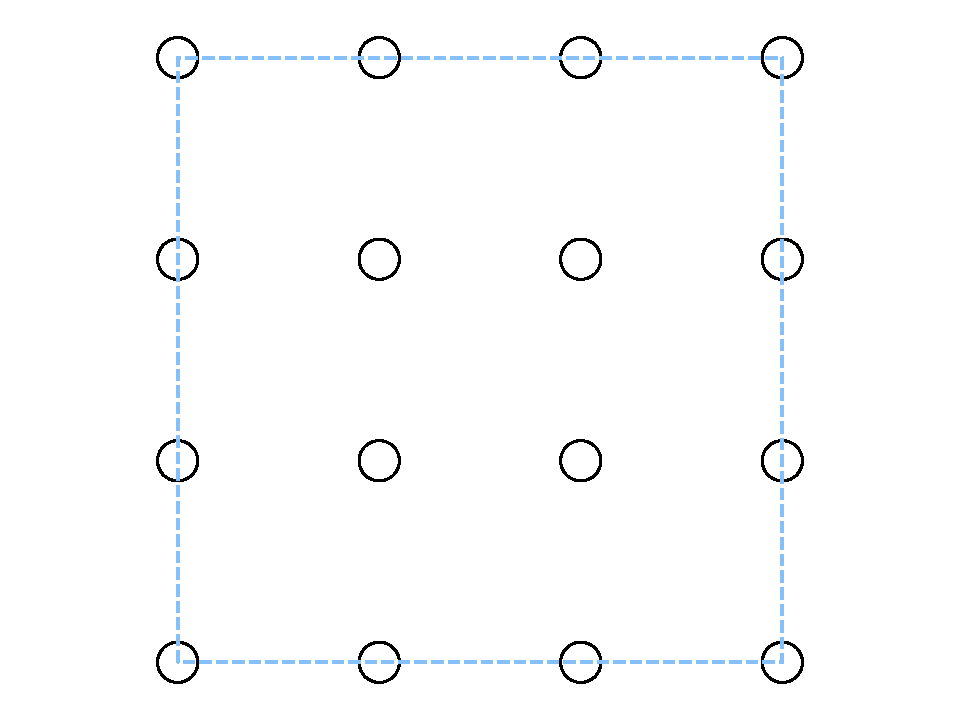
\includegraphics[width=1.\textwidth, trim={1.5cm, 0cm, 1.5cm, 0cm}, clip]{final_images/layouts/16_turb_start.pdf}
\caption{Baseline wind farm layout for case 1. The circles marking turbine locations are to scale, with diameters equal to the rotor diameter.}
\label{fig:grid_case}
\end{minipage}\hspace{1pc}%
\begin{minipage}[t]{18pc}
\centering
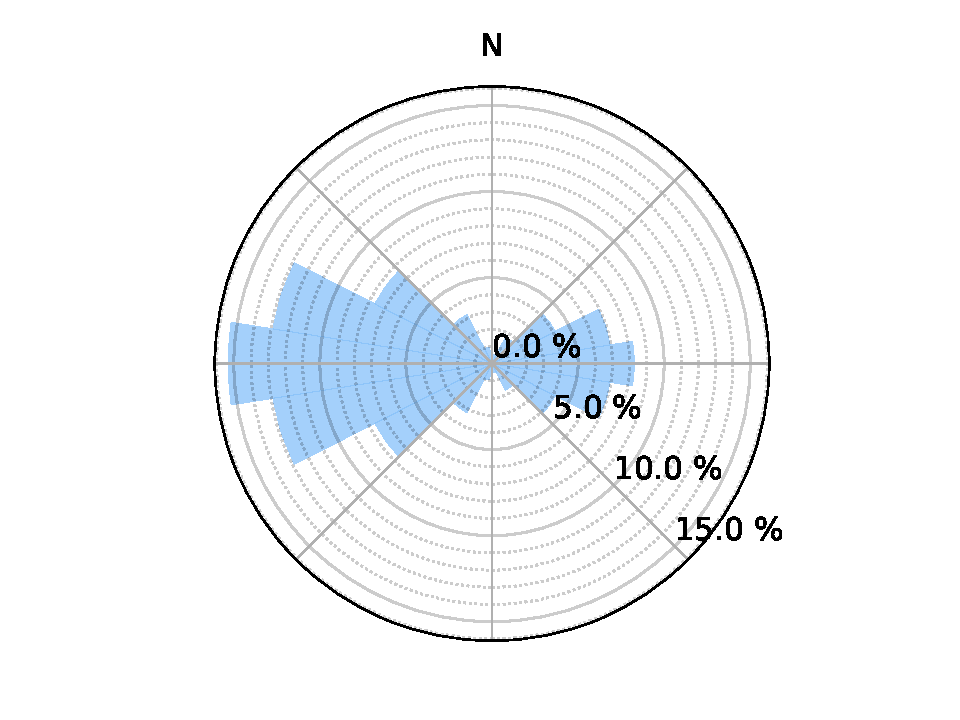
\includegraphics[width=\textwidth, trim={2.0cm 0cm 2.0cm 0cm}, clip]{final_images/windroses/freqwindrose_20_dir.pdf}
\caption{Direction probability wind rose for case 1. This wind rose is composed of a double Gaussian distribution binned into 20 directions.}
\label{fig:directional}
\end{minipage} 
\end{figure}
%

For case 1, the optimization problem was formulated as shown in \cref{eqn:opt1}
%
\begin{equation}
	\label{eqn:opt1}
	\begin{aligned} [b]
	\underset{x_i,y_i}{\textrm{maximize}} \quad & AEP(x_i,y_i,)~~i=1...16\\
	\textrm{subject to} \quad & s_{i,j} \geq 2\*d~~i,j=1...16,~~i \neq j\\
	 & x_{min} \leq x_i \leq x_{max}~~i=1...16\\
     & y_{min} \leq y_i \leq y_{max}~~i=1...16
	\end{aligned}
\end{equation}
%
Where $x_{max/min}$ and $y_{max/min}$ represent the boundaries of the wind farm. This case has a total of 32 variables and 120 constraints.

\subsection{Case 2: Round Farm}

  Case 2 was created to be significantly more challenging than the first case, but still fairly simple. We defined a wind farm with 38 wind turbines and a circular boundary as shown in \cref{fig:round_case}. 
%
\begin{figure}[h!]
	\centering
	\begin{minipage}[t]{18pc}
		\centering
		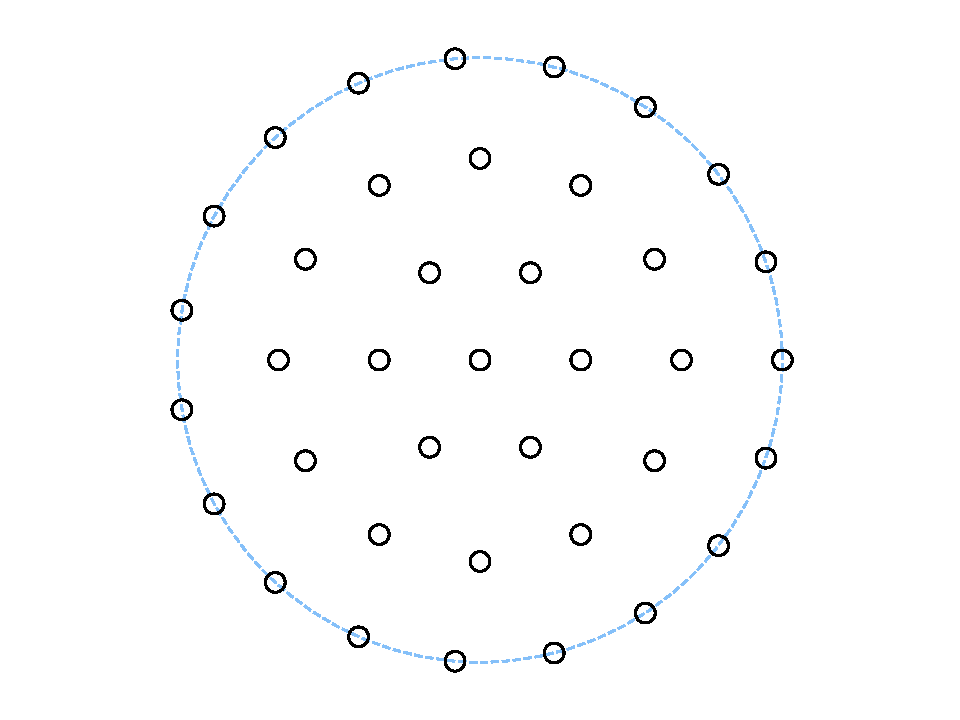
\includegraphics[width=\textwidth, trim={1.5cm, 0cm, 1.5cm, 0cm}, clip]{final_images/layouts/38_turb_start.pdf}
		\caption{Baseline wind farm layout for case 2. The circles marking turbine locations are to scale, with diameters equal to the rotor diameter.}
		\label{fig:round_case}
	\end{minipage}\hspace{1pc}%
\end{figure}
%
The size of the boundary allowed for at least a five-diameter spacing between turbines. We used the Nantucket wind rose binned into 36 directions with the wind speed for each direction determined as the average of all samples in that sector as shown in \cref{fig:speedwindrose_36dir,fig:freqwindrose_36dir}.
%
\begin{figure}[h!]
\centering
\begin{minipage}[t]{18pc}
\centering
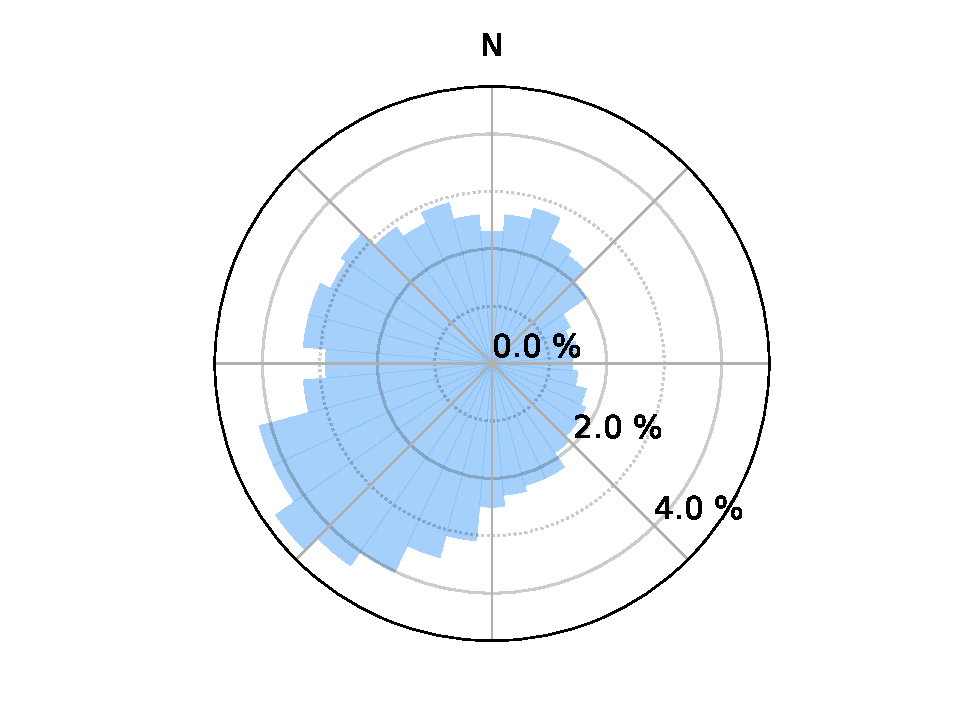
\includegraphics[width=\textwidth, trim={1.5cm 0cm 1.5cm 0cm}, clip]{final_images/windroses/freqwindrose_36_dir.pdf}
\caption{Directional probability wind rose for case 2. This is the Nantucket wind rose binned into 36 directions \cite{wrcc2017}.}
\label{fig:freqwindrose_36dir}
\end{minipage} \hspace{1pc}%
\begin{minipage}[t]{18pc}
	\centering
	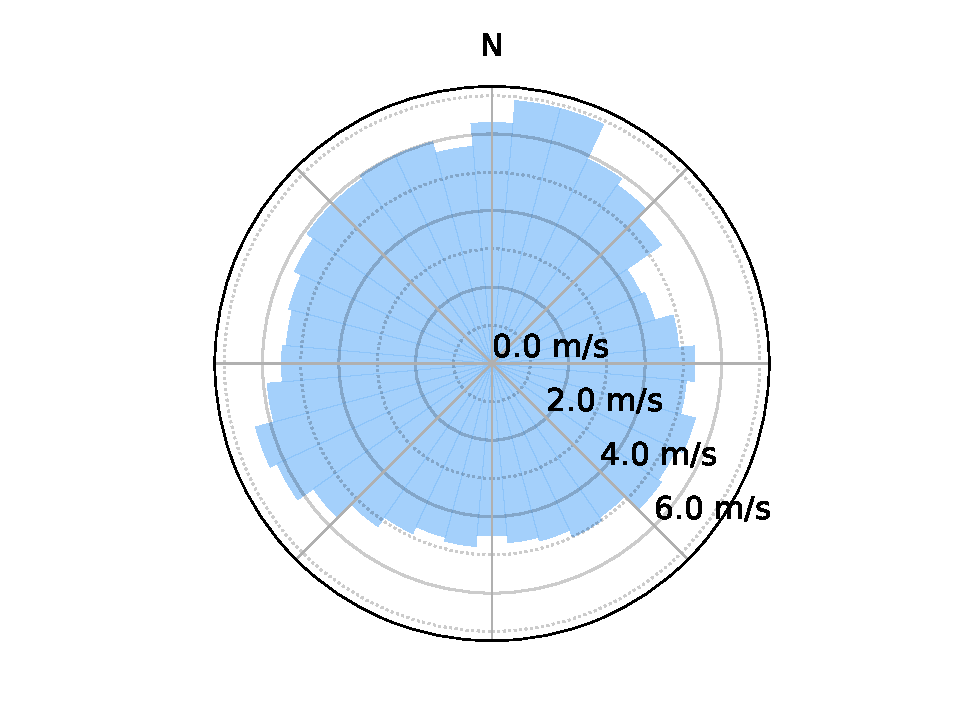
\includegraphics[width=\textwidth, trim={1.5cm, 0cm, 1.5cm, 0cm}, clip]{final_images/windroses/speedwindrose_36_dir.pdf}
	\caption{Average speed wind rose for case 2. This is the Nantucket wind rose binned into 36 directions \cite{wrcc2017}}
	\label{fig:speedwindrose_36dir}
\end{minipage}
\end{figure}

The optimization problem for case 2 was formulated as
%
\begin{equation}
	\label{e:objective}
	\begin{aligned} [b]
	\underset{x_i,y_i}{\textrm{maximize}} \quad & AEP(x_i,y_i,)~~i=1...38\\
	\textrm{subject to} \quad & s_{i,j} \geq 2\*d~~i,j=1...38~~i \neq j\\
	 & [x_c-x_i]^2+[y_c-y_i]^2 \leq r_{b}^2~~i=1...38
	\end{aligned}
\end{equation}
%
Case 2 has a total of 76 variables and 741 constraints.

\subsection{Case 3: Princess Amalia Wind Farm}
Case 3 was selected to provide a larger and somewhat more realistic problem. The Amalia wind farm has 60 wind turbines. We used the convex hull of the existing turbine locations to create a convex polygonal boundary. We used wind data binned into 72 wind directions with wind speed for each direction determined as the average of all samples in that sector as shown in \cref{fig:speedwindrose_72dir,fig:freqwindrose_72dir}
\begin{figure}[h!]
	\centering
	\begin{minipage}[t]{18pc}
		\centering
		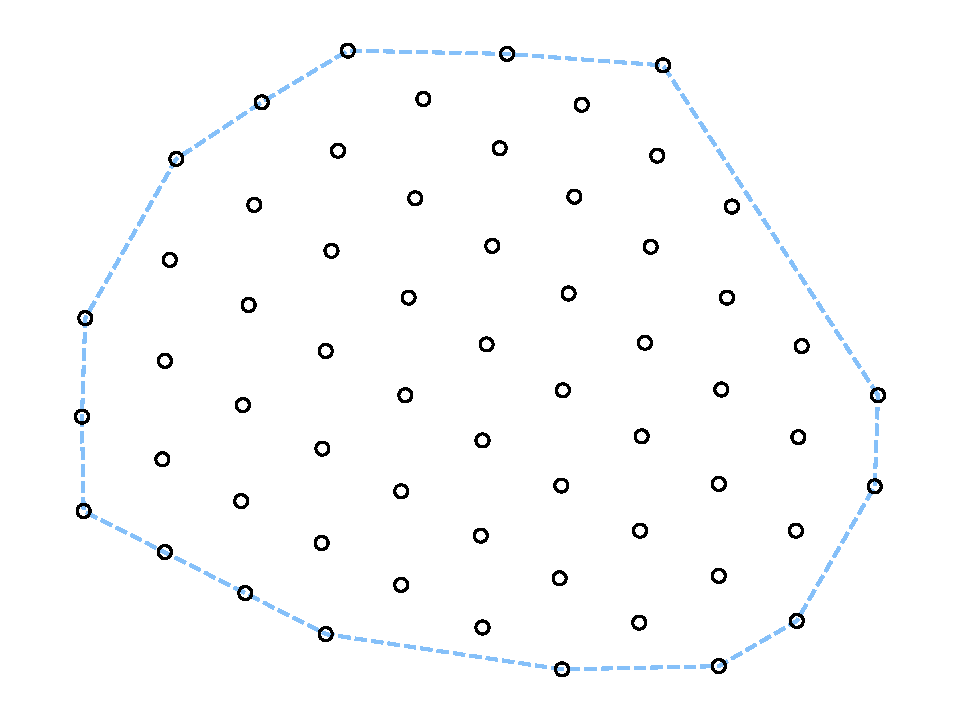
\includegraphics[width=1.\textwidth, trim={1.0cm, 0cm, 1.0cm, 0cm}, clip]{final_images/layouts/60_turb_start.pdf}
		\caption{Baseline wind farm layout for case 3. The circles marking turbine locations are to scale, with diameters equal to the rotor diameter.}
		\label{fig:amalia_base_layout}
	\end{minipage}\hspace{1pc}%
\end{figure}

\begin{figure}[h!]
	\centering
	\begin{minipage}[t]{18pc}
		\centering
		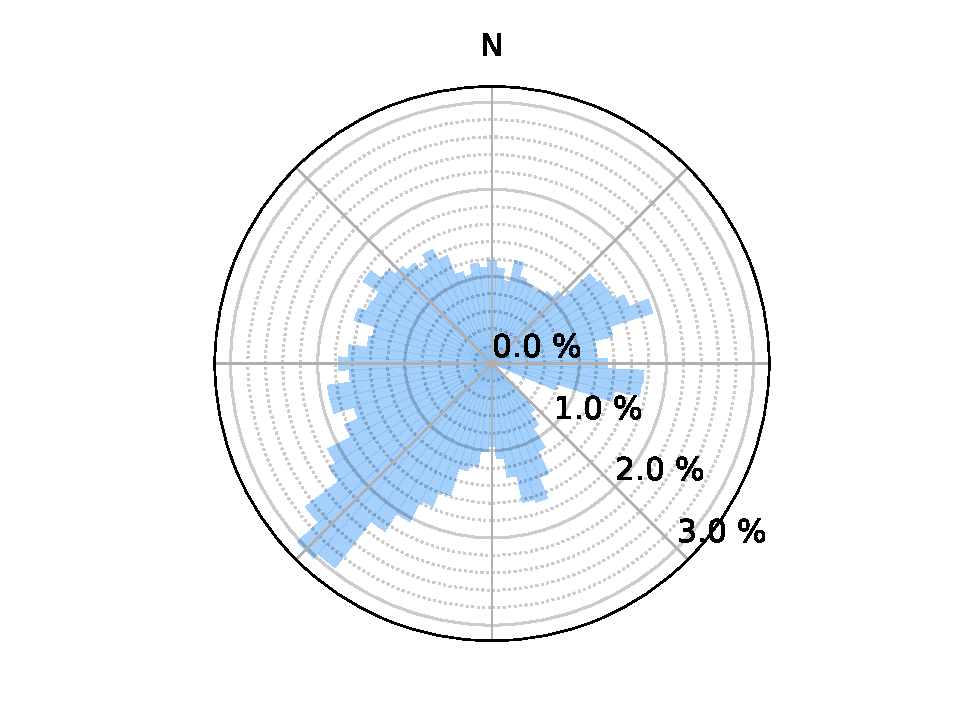
\includegraphics[width=\textwidth, trim={1.5cm 0cm 1.5cm 0cm}, clip]{final_images/windroses/freqwindrose_72_dir.pdf}
		\caption{Direction probability wind rose for case 3. The wind rose is comprised of data from \cite{noordzeewind2006}. Measurements were taken from July 1, 2005, to June 30, 2006.}
		\label{fig:freqwindrose_72dir}
	\end{minipage} \hspace{1pc}%
	\begin{minipage}[t]{18pc}
		\centering
		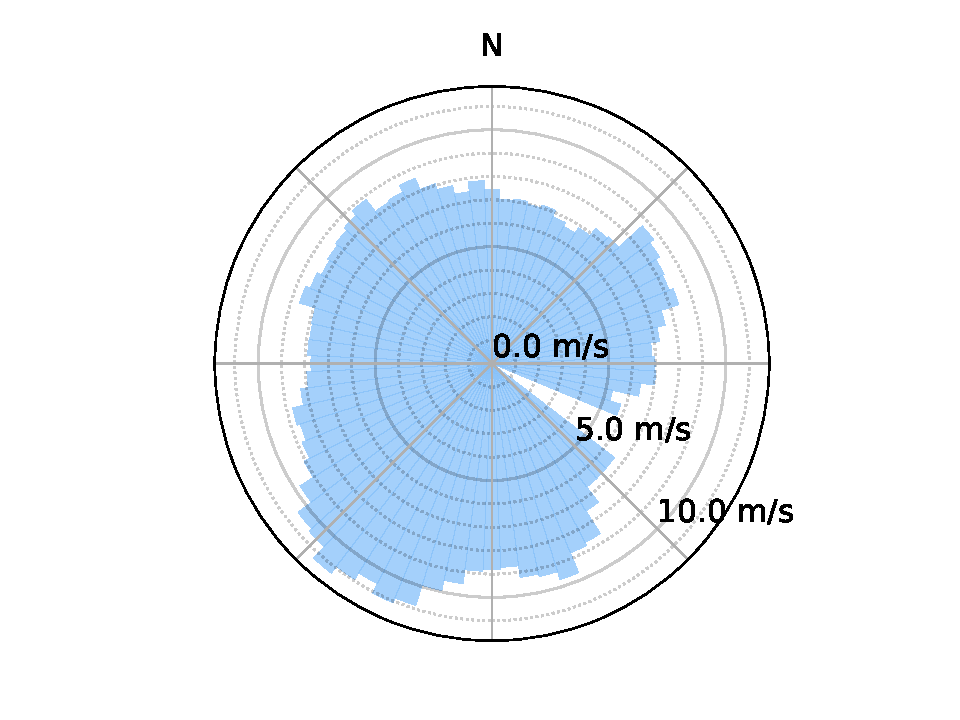
\includegraphics[width=1.\textwidth, trim={1.5cm, 0cm, 1.5cm, 0cm}, clip]{final_images/windroses/speedwindrose_72_dir.pdf}
		\caption{Average speed wind rose for case 3. The wind rose is comprised of data from \cite{noordzeewind2006}. Measurements were taken from July 1, 2005, to June 30, 2006.}
		\label{fig:speedwindrose_72dir}
	\end{minipage}
\end{figure}
%
For case 3, the optimization problem was formulated as shown in \cref{eqn:opt3}
%
\begin{equation}
\label{eqn:opt3}
\begin{aligned} [b]
\underset{x_i,y_i}{\textrm{maximize}} \quad & AEP(x_i,y_i,)~~i=1...60\\
\textrm{subject to} \quad & s_{i,j} \geq 2\*d~~i,j=1...60,~~i \neq j\\
& b_{i,k} \geq 0 ~~ i=1...60, k=1...14
\end{aligned}
\end{equation}
%
Where $b_{i,k}$ represents the distance of each turbine $i$ from each boundary $k$. Case 3 has a total of 120 variables and 2610 constraints.

\section{Results and Discussion}\label{sec:resultsanddiscussion}
%\todo{Jared: figure out how to best present these results now that we have 3 models}
We compared wake loss and the number of function calls required for each of the cases discussed previously. We also performed a Welch's t-test between the SNOPT and SNOPT+WEC results. We used function calls as a surrogate for time. We did not report wall time because we did not maintain enough consistency in the computational resources used for each optimization run (cores, processor types, computational isolation, etc). 

Results for case 1 are shown in \cref{fig:case-1-wake-loss,fig:case-1-fcalls,tab:case1}. Results for case 2 are presented in \cref{fig:case-2-wake-loss,fig:case-2-wake-loss-no-outliers,fig:case-2-fcalls,tab:case2}.  Results for case 3 are presented in \cref{fig:case-3-wake-loss,fig:case-3-wake-loss-no-outliers,fig:case-3-fcalls,tab:case3}. 
%
%\begin{figure}[h!]  
%\centering
%\begin{minipage}[t]{18pc}    
%\centering
%\includegraphics[width=\textwidth, trim={0cm 0cm 0cm 0cm}]{final_images/results/16turbs_results_alpso_percent_wake_loss.pdf}
%\caption{Box plot comparing the wake loss results across each optimization approach for case 1 (16 turbines)}
%\label{fig:case-1-wake-loss}
%\end{minipage}\hspace{1pc} 
%\centering
%\begin{minipage}[t]{18pc}    
%	\centering
%	\includegraphics[width=\textwidth]{final_images/results/16turbs_results_alpso_fcalls.pdf}
%	\caption{Box plot comparing the number of function calls used by each optimization approach for case 1 (16 turbines)}
%	\label{fig:case-1-fcalls}
%\end{minipage}
%\end{figure}
%
\begin{figure}[h]
\centering
\begin{minipage}[t]{.75\textwidth}
\centering
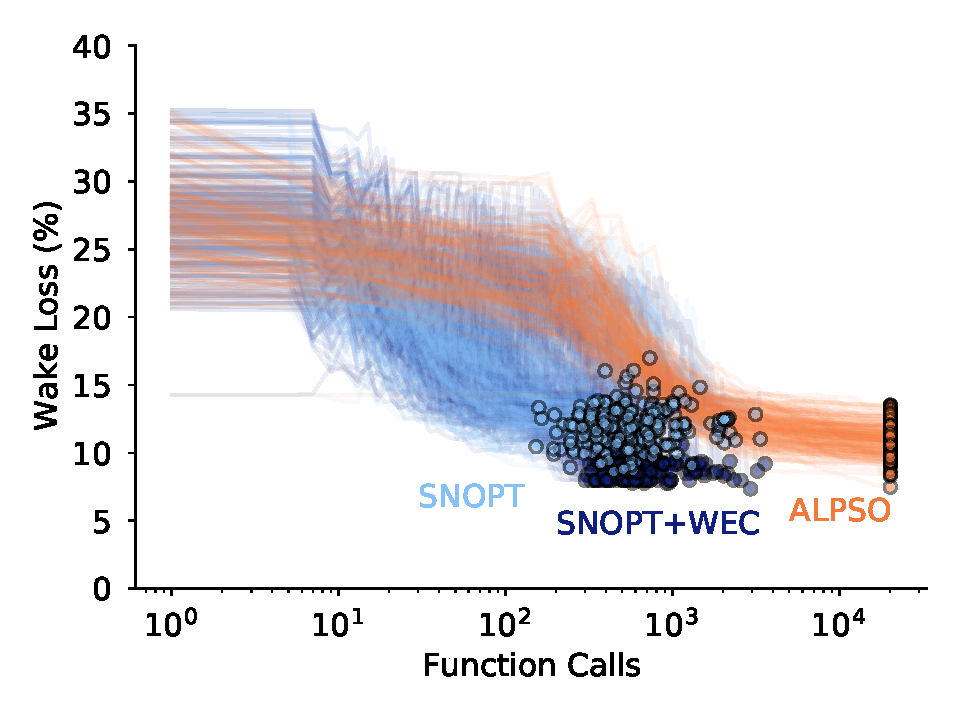
\includegraphics[width=\textwidth]{final_images/results/convergence_history_BPAmodel_16turbs_20dirs}  
\caption{Convergence histories of optimizations run from 200 different starting points for case 1 (16 turbines) using three different optimization approaches. Markers indicate optimized values.}
\label{fig:case-1-histories}
\end{minipage} 
\end{figure}
%
\begin{table}
	\centering
	\caption{Optimization Results for BPA Model: 16 Turbines, 20 Directions}
	\label{tab:case1}
	\begin{tabular}{lrrrrrrrrr}
		\toprule
		{} & \multicolumn{3}{c}{Function Calls} & \multicolumn{6}{c}{Wake Loss (\%)} \\
		\cmidrule(lr){2-4} \cmidrule(lr){5-10}
		{} &         Median &    Low &   High &        Median &   Mean &    SD &   Low &   High &          p \\
		\cmidrule(lr){2-4} \cmidrule(lr){5-10}
		SNOPT     &            547 &      0 &   3352 &        11.885 & 11.872 & 1.473 & 8.630 & 16.988 &            \\
		SNOPT+WEC &            625 &      0 &   3594 &         9.169 &  8.858 & 0.703 & 7.346 & 12.137 &  $< 0.001$ \\
		ALPSO     &          20132 &  20132 &  20132 &        10.951 & 10.940 & 1.094 & 7.479 & 13.523 &            \\
		\bottomrule
	\end{tabular}
\end{table}
%\begin{table}
%\caption{Optimization Results for Case 1}
%\label{tab:case1}
%\centering
%\begin{tabular}{lcrrrcrrrrrr}
%	\br
%	& & \multicolumn{3}{c}{Function Calls} &  & \multicolumn{6}{c}{\quad \quad \quad \quad \quad Wake Loss (\%) \quad \quad \quad \quad \quad} \\
%	\cline{3-5}\cline{7-12}
%	Method  & & Median & Low & High & & Mean & SD & Low & High & $p$ \\
%	\cline{1-1}\cline{3-5}\cline{7-12}
%	SNOPT  & & 550.0 & 156 & 3352 & & 11.88 & 1.42 & 8.32 & 15.56 &   \\
%	SNOPT+WEC & & 2,563.5 & 745.0 & 4,487.0 &  &  9.04 & 0.90 & 7.41 & 11.77 & $<.001$\\
%	ALPSO & & 71,652.0 & 5,277.0 & 136,527.0 & & 13.49 & 1.50 & 10.77 & 16.68 & \\
%	\br
%\end{tabular}
%\end{table}


%
%\begin{figure}[h]  
%	\centering
%	\begin{minipage}[t]{0.48\textwidth}    
%		\centering
%		\includegraphics[width=\textwidth, trim={0cm 0cm 0cm 0cm}]{final_images/results/38turbs_results_alpso_percent_wake_loss.pdf}
%		\caption{Box plot comparing the wake loss results across each optimization approach for case 2 (38 turbines)}
%		\label{fig:case-2-wake-loss}
%	\end{minipage}\hspace{1pc}
%	\begin{minipage}[t]{0.48\textwidth}    
%		\centering
%		\includegraphics[width=\textwidth, trim={0cm 0cm 0cm 0cm}]{final_images/results/38turbs_results_alpso_percent_wake_loss_zoom.pdf}
%		\caption{Box plot comparing the wake loss results across each optimization approach for case 2 (38 turbines) with outliers removed}
%		\label{fig:case-2-wake-loss-no-outliers}
%	\end{minipage}
%\end{figure}

%\begin{figure}[h]
%\centering
%\begin{minipage}[t]{18pc}
%\centering
%\includegraphics[width=\textwidth]{final_images/results/38turbs_results_alpso_fcalls}  
%\caption{Box plot comparing the number of function calls used by each optimization approach for case 2 (38 turbines)}
%\label{fig:case-2-fcalls}
%\end{minipage} 
%\end{figure}
%
\begin{figure}[h]
	\centering
	\begin{minipage}[t]{.75\textwidth}
		\centering
		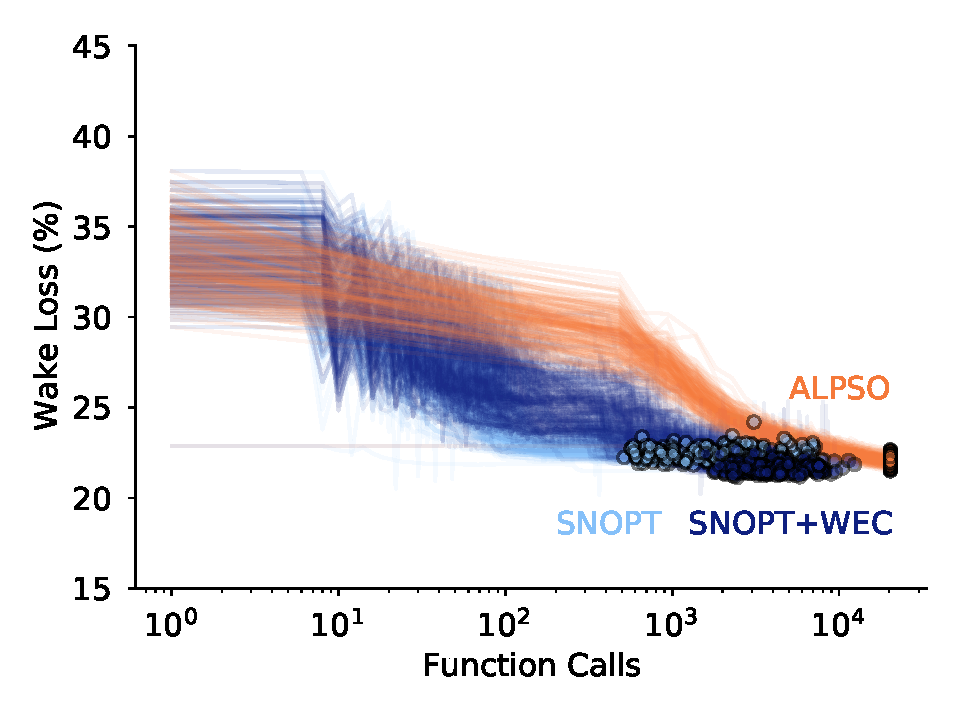
\includegraphics[width=\textwidth]{final_images/results/convergence_history_BPAmodel_38turbs_36dirs}  
		\caption{Convergence histories of optimizations run from 200 different starting points for case 2 (38 turbines) using three different optimization approaches. Markers indicate optimized values.}
		\label{fig:case-2-histories}
	\end{minipage} 
\end{figure}
%
%\begin{table}[h]
%  \caption{Optimization Results for Case 2}
%  \label{tab:case2}
%  \centering
%  \begin{tabular}{lcrrrcrrrrrr}
%  \br
%   & & \multicolumn{3}{c}{Function Calls} &  & \multicolumn{6}{c}{\quad \quad \quad \quad \quad Wake Loss (\%) \quad \quad \quad \quad \quad } \\
%   \cline{3-5}\cline{7-12} 
%%   \vspace{1pt} 
%  Method  & & Med. & Low & High & & Mean & SD & Low & High & $p$\\
%   \cline{1-1}\cline{3-5}\cline{7-12}
%  SNOPT  & & 1,847.0 & 166.0 & 8,618.0 & & 23.72 & 1.00 & 22.78 & 36.64  &  \\
%  SNOPT+WEC & & 4,102.0 & 1,183.0 & 10,653.0 &  &  22.80 & 0.37 & 22.02 & 23.96 & $< .001$ \\
%  ALPSO & & 3,338.0 & 170.0 & 9,242.0 & & 26.08 & 0.95 & 22.89 & 31.89 & \\
%  \br
%  \end{tabular}
%\end{table}
%\begin{table}
%	\centering
%	\caption{Optimization Results for BPA Model: 38 Turbines, 12 Directions}
%	\begin{tabular}{lrrrrrrrrr}
%		\toprule
%		{} & \multicolumn{3}{c}{Function Calls} & \multicolumn{6}{c}{Wake Loss (\%)} \\
%		{} &         Median &    Low &   High &        Median &   Mean &    SD &    Low &   High &          p \\
%		\midrule
%		SNOPT     &            595 &    206 &   2224 &        16.304 & 16.338 & 0.790 & 14.505 & 19.102 &            \\
%		SNOPT+WEC &           2693 &    828 &  10710 &        13.285 & 13.280 & 0.341 & 11.725 & 14.035 &  $< 0.001$ \\
%		ALPSO     &          21032 &  21032 &  21032 &        15.076 & 15.097 & 0.555 & 13.658 & 17.016 &            \\
%		ALPSO+WEC &           3782 &   3782 &   3782 &        14.098 & 14.096 & 0.425 & 12.532 & 15.762 &  $< 0.001$ \\
%		\bottomrule
%	\end{tabular}
%\end{table}
\begin{table}
	\centering
	\caption{Optimization Results for BPA Model: 38 Turbines, 12 Directions}
	\begin{tabular}{lrrrrrrrrr}
		\toprule
		{} & \multicolumn{3}{c}{Function Calls} & \multicolumn{6}{c}{Wake Loss (\%)} \\
		\cmidrule(lr){2-4} \cmidrule(lr){5-10}
		{} &         Median &    Low &   High &        Median &   Mean &    SD &    Low &   High &          p \\
		\cmidrule(lr){2-4} \cmidrule(lr){5-10}
		SNOPT     &            595 &    206 &   2224 &        16.304 & 16.338 & 0.790 & 14.505 & 19.102 &            \\
		SNOPT+WEC &           2693 &    828 &  10710 &        13.285 & 13.280 & 0.341 & 11.725 & 14.035 &  $< 0.001$ \\
		ALPSO     &          21032 &  21032 &  21032 &        15.076 & 15.097 & 0.555 & 13.658 & 17.016 &            \\
		ALPSO+WEC &          26474 &  26474 &  26474 &        14.098 & 14.096 & 0.425 & 12.532 & 15.762 &  $< 0.001$ \\
		\bottomrule
	\end{tabular}
\end{table}
\begin{table}
	\centering
	\caption{Optimization Results for BPA Model: 38 Turbines, 36 Directions}
	\label{tab:case2}
	\begin{tabular}{lrrrrrrrrr}
		\toprule
		{} & \multicolumn{3}{c}{Function Calls} & \multicolumn{6}{c}{Wake Loss (\%)} \\
		\cmidrule(lr){2-4} \cmidrule(lr){5-10}
		{} &         Median &    Low &   High &        Median &   Mean &    SD &    Low &   High &          p \\
		\cmidrule(lr){2-4} \cmidrule(lr){5-10}
		SNOPT     &           1985 &      0 &   7768 &        22.417 & 22.439 & 0.370 & 21.487 & 24.203 &            \\
		SNOPT+WEC &           3706 &    330 &  12382 &        21.588 & 21.646 & 0.292 & 21.147 & 22.680 &  $< 0.001$ \\
		ALPSO     &          20282 &  20282 &  20282 &        22.062 & 22.075 & 0.231 & 21.510 & 22.667 &            \\
		\bottomrule
	\end{tabular}
\end{table}
%
%\begin{figure}[h!]  
%	\centering
%	\begin{minipage}[t]{0.48\textwidth}    
%		\centering
%		\includegraphics[width=\textwidth, trim={0cm 0cm 0cm 0cm}]{final_images/results/60turbs_results_alpso_percent_wake_loss.pdf}
%		\caption{Box plot comparing the wake loss results across each optimization approach for case 3 (60 turbines)}
%		\label{fig:case-3-wake-loss}
%	\end{minipage}\hspace{1pc}
%	\begin{minipage}[t]{0.48\textwidth}    
%		\centering
%		\includegraphics[width=\textwidth, trim={0cm 0cm 0cm 0cm}]{final_images/results/60turbs_results_alpso_percent_wake_loss_zoom.pdf}
%		\caption{Box plot comparing the wake loss results across each optimization approach for case 3 (60 turbines) with outliers removed}
%		\label{fig:case-3-wake-loss-no-outliers}
%	\end{minipage}
%\end{figure}
%
%
%\begin{figure}[h]
%	\centering
%	\begin{minipage}[t]{18pc}
%		\centering
%		\includegraphics[width=\textwidth]{final_images/results/60turbs_results_alpso_fcalls}  
%		\caption{Box plot comparing the number of function calls used by each optimization approach for case 3 (60 turbines)}
%		\label{fig:case-3-fcalls}
%	\end{minipage} 
%\end{figure}
%
%%
\begin{figure}[h]
	\centering
	\begin{minipage}[t]{.75\textwidth}
		\centering
		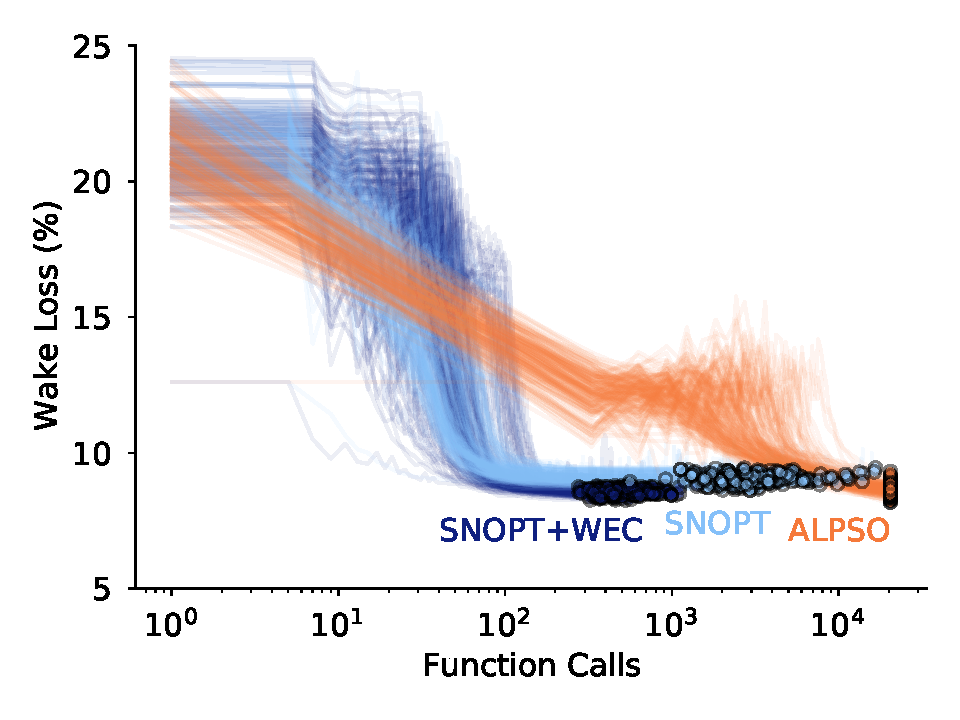
\includegraphics[width=\textwidth]{final_images/results/convergence_history_BPAmodel_60turbs_72dirs}  
		\caption{Convergence histories of optimizations run from 200 different starting points for case 3 (60 turbines) using three different optimization approaches. Markers indicate optimized values.}
		\label{fig:case-3-histories}
	\end{minipage} 
\end{figure}
%
%\begin{table}[h]
%	\caption{Optimization Results for Case 3}
%	\label{tab:case3}
%	\centering
%	\begin{tabular}{lcrrrcrrrrrr}
%		\br
%		& & \multicolumn{3}{c}{Function Calls} &  & \multicolumn{6}{c}{\quad \quad \quad \quad \quad Wake Loss (\%) \quad \quad \quad \quad \quad} \\
%		\cline{3-5}\cline{7-12}
%		Method  & & Med. & Low & High & & Mean & SD & Low & High & $p$\\
%		\cline{1-1}\cline{3-5}\cline{7-12}
%		SNOPT  & & 4,415.0 & 254.0 & 20,318.0 & & 10.07 & 1.55 & 9.41 & 21.90 &  \\
%		SNOPT+WEC & & 12,970.0 & 5045.0& 34,565.0 &  &  9.30 & 0.13 & 8.90 & 9.90 & $<.001$ \\
%	    ALPSO & & 2042.0 & 170.0 & 6,218.0 & & 10.33 & 0.39 & 9.52 & 12.62 &\\
%		\br
%	\end{tabular}
%\end{table}
\begin{table}
	\centering
	\caption{Optimization Results for BPA Model: 60 Turbines, 72 Directions}
	\begin{tabular}{lrrrrrrrrr}
		\toprule
		{} & \multicolumn{3}{c}{Function Calls} & \multicolumn{6}{c}{Wake Loss (\%)} \\
		\cmidrule(lr){2-4} \cmidrule(lr){5-10}
		{} &         Median &    Low &   High &        Median &  Mean &    SD &   Low &  High &          p \\
		\cmidrule(lr){2-4} \cmidrule(lr){5-10}
		SNOPT     &           2701 &      0 &  16644 &         9.033 & 9.041 & 0.176 & 8.625 & 9.445 &            \\
		SNOPT+WEC &            483 &    180 &   1424 &         8.540 & 8.551 & 0.118 & 8.260 & 8.830 &  $< 0.001$ \\
		ALPSO     &          20432 &  20432 &  20432 &         8.632 & 8.647 & 0.185 & 8.183 & 9.314 &            \\
		\bottomrule
	\end{tabular}
\end{table}

In the more general WFLO problem, we are looking for high AEP values, a tight distribution, and relatively few function calls. The benefit of high AEP means that the resulting wind farm will be more efficient, likely leading to a reduced cost of energy. A tight distribution means that the method is consistent, that the optimized solution is independent of the starting layout. The tighter the distribution the fewer optimizations need to be run before we are confident that we have one of the best wind farm designs we can get. A low number of function calls means that wind farm design can be done more cheaply and that more variables could potentially be tested, which could again lead to a lower cost of energy. Each of the methods tested demonstrated at least one of these characteristics.

The relatively low wake loss results from ALPSO on the smaller case, compared to the relatively high wake loss results of ALPSO on larger case illustrates an inherent weakness of gradient-free algorithms. Namely, that increased dimensionality generally leads to a decrease in the performance of gradient-free algorithms \cite{rios2013-grad-free-comparison}.

The relatively wide spread and moderate results from SNOPT on both cases demonstrate one of the weaknesses of gradient-based algorithms. While gradient-based algorithms tend to need fewer function calls, and thus typically less time, they are highly susceptible to local optima. That WEC wake loss results were lower and less spread for all test cases, as compared with SNOPT, seems to indicate that the process is at least partially remedying the problem of local optima.

The low values of wake loss and lower standard deviation of wake loss for SNOPT with WEC, indicates that SNOPT with WEC is more accurate and reliable than SNOPT alone. So much so that, ignoring outliers, the probability distributions for SNOPT with and without WEC from case 3 overlap only slightly (see \cref{fig:case-3-wake-loss-no-outliers}). This improvement in performance does come at the cost of more function calls than SNOPT without WEC. The increase in function calls when using WEC is expected because the WEC ran seven optimizations to convergence (one for each value of $\xi$, and a final optimization to account for local turbulence intensity) for every one optimization by SNOPT alone. Because WEC has a smaller probability distribution than SNOPT by itself, fewer runs would be needed to gain the same level of confidence in the results. The reduction in overall runs could mean an overall reduction in the number of function evaluations for WEC as compared to SNOPT alone.

\section{Conclusion}
The WEC method proposed in this paper uses characteristics of typical wake models to reduce the multi-modal nature of the design space. We tested three versions of WEC on a simple wind farm and tested the final version of WEC with two wake models and three WFLO problems, one with 16 turbines, one with 38 turbines, and one with 60 turbines. Results for the case studies using WEC show a statistically significant reduction  (p<.001) in optimized wake loss compared to gradient-based optimization without WEC and gradient-free optimization for all test cases.

Future work should investigate potential improvements and best practices for WEC to reduce the number of function calls required, provide a more complete comparison to gradient-free wind farm layout optimization including discrete parameterization, and validate the results obtained through WEC using a higher-order modeling approach such as Large Eddy Simulation (LES).

\ack 
This work was supported by the National Science Foundation under Grant No. 1539384. Any opinions, findings, and conclusions or recommendations expressed in this material are those of the authors and do not necessarily reflect the views of the National Science Foundation.

\section*{References}
\bibliographystyle{iopart-num}
\bibliography{./references/all_refs}

\end{document}

